% ============================================================
% Chapter 6: Markov Chain Monte Carlo Methods
% Lectures on Monte Carlo Theory — Leskelä & Vihola (Lorek & Rolski)
% Reader-friendly version: complete sentences, full derivations,
% worked examples. Every symbol is defined. Self-contained.
% ============================================================
\documentclass[aspectratio=169,10pt]{beamer}
\usetheme{Madrid}
\usecolortheme{seahorse}

\usepackage{amsmath,amssymb,amsthm}
\usepackage{mathtools}
\usepackage{bm}
\usepackage{xcolor}
\usepackage{booktabs}
\usepackage{graphicx}
\usepackage{listings}
\usepackage{tikz}
\usepackage{enumerate}
\usetikzlibrary{arrows.meta,positioning,shapes}

\graphicspath{{figures/}}

\lstdefinestyle{python}{
  language=Python,
  basicstyle=\ttfamily\scriptsize,
  numbers=left,
  numberstyle=\tiny\color{gray},
  frame=single,
  backgroundcolor=\color{gray!7},
  keywordstyle=\color{blue!70!black}\bfseries,
  commentstyle=\color{green!50!black}\itshape,
  stringstyle=\color{red!60!black},
  breaklines=true,
  showstringspaces=false,
  tabsize=4,
}

\setbeamertemplate{footline}[frame number]
\setbeamertemplate{navigation symbols}{}

\newcommand{\PP}{\mathbb{P}}
\newcommand{\EE}{\mathbb{E}}
\newcommand{\RR}{\mathbb{R}}
\newcommand{\ZZ}{\mathbb{Z}}
\newcommand{\dTV}{d_{\mathrm{TV}}}
\newcommand{\bfP}{\mathbf{P}}
\newcommand{\bfQ}{\mathbf{Q}}
\newcommand{\bfC}{\mathbf{C}}
\newcommand{\bfZ}{\mathbf{Z}}
\newcommand{\bff}{\mathbf{f}}
\newcommand{\bfpi}{\bm{\pi}}
\newcommand{\bfmu}{\bm{\mu}}

\title[Chapter 6: MCMC]{Chapter 6: Markov Chain Monte Carlo Methods}
\subtitle{Lectures on Monte Carlo Theory --- Lorek \& Rolski}
\author{}
\date{}

% ============================================================
\begin{document}
% ============================================================

\begin{frame}
  \titlepage
\end{frame}

\begin{frame}{Chapter Overview}
  \tableofcontents
\end{frame}

% ============================================================
\section{6.1 Introduction}
% ============================================================

\begin{frame}[allowframebreaks]{6.1 Introduction: The Problem with Direct Sampling}

In previous chapters the goal was to estimate
\[
  I = \EE Y \quad \text{or} \quad I = \EE f(Y),
\]
where $Y$ follows a prescribed distribution $\pi$ on some state space $\mathcal{S}$.
The standard Monte Carlo approach generates $R$ independent samples $Y_1, \ldots, Y_R \sim \pi$ and uses the sample mean
\[
  \hat{Y}_R = \frac{1}{R} \sum_{i=1}^{R} f(Y_i) \approx I.
\]
This works beautifully when $\pi$ is easy to sample from.

\medskip
However, in many real problems the target distribution $\pi$ is \emph{intractable}:

\begin{block}{Two Sources of Intractability}
\begin{enumerate}
  \item The state space $\mathcal{S}$ is \textbf{combinatorially large}: for example, $|\mathcal{S}| = 2^d$ grows exponentially in the problem dimension $d$, making enumeration hopeless.
  \item The distribution $\pi$ involves an \textbf{unknown normalising constant}: $\pi_\sigma = e^{\lambda f(\sigma)}/z_\lambda$, where $z_\lambda = \sum_\sigma e^{\lambda f(\sigma)}$ cannot be computed.
\end{enumerate}
\end{block}

\framebreak

\textbf{Running example.} Consider the set $\mathcal{S}_n$ of all permutations of $n$ elements.
A random permutation $Y \sim \pi_n$ is drawn uniformly, i.e.\ $\pi_\sigma = 1/n!$ for every $\sigma \in \mathcal{S}_n$.
The function of interest counts fixed points: $f(\sigma) = \#\{i : \sigma(i) = i\}$.
In this uniform case direct sampling is easy (Fisher-Yates algorithm), and we simply average $f$ over the samples.

Now complicate the scenario by making $\pi$ non-uniform:
\[
  \pi_\sigma = \frac{1}{z_\lambda} \exp(\lambda f(\sigma)), \qquad z_\lambda = \sum_{\sigma \in \mathcal{S}_n} \exp(\lambda f(\sigma)).
\]
Here $\lambda$ is a real parameter controlling how strongly we weight permutations with many fixed points.
Computing $z_\lambda$ requires summing over all $n!$ permutations, which is completely infeasible for large $n$.

\begin{alertblock}{Key Insight: MCMC}
The \textbf{Markov Chain Monte Carlo} (MCMC) paradigm resolves this by constructing a Markov chain $(X_n)_{n \ge 0}$ on $\mathcal{S}$ whose \emph{stationary distribution} is exactly $\pi$.
The ergodic theorem then guarantees
\[
  \hat{Y}_R = \frac{1}{R} \sum_{j=1}^{R} f(X_j) \xrightarrow{R \to \infty} I \quad \text{almost surely.}
\]
Crucially, only \emph{ratios} $\pi_{s'}/\pi_s = e^{\lambda(f(s')-f(s))}$ are needed; the constant $z_\lambda$ cancels!
\end{alertblock}

MCMC allows us to achieve two goals:
\begin{enumerate}
  \item[(A1)] Generate approximate (or in some cases exact) samples from $\pi$.
  \item[(A2)] Estimate probabilities $\pi(A) = \sum_{s \in A} \pi_s$ for subsets $A \subseteq \mathcal{S}$.
\end{enumerate}

\end{frame}

% ============================================================
\section{6.2 Markov Chains}
% ============================================================

\begin{frame}[allowframebreaks]{6.2 Markov Chains: Core Definitions}

A \emph{Markov chain} is a sequence of random variables $(X_n)_{n \ge 0}$ that evolves on a \emph{finite} state space $\mathcal{S} = \{s_1, \ldots, s_N\}$ according to the Markov (memoryless) property.

\begin{block}{Definition: Markov Chain and Transition Matrix}
The sequence $(X_n)_{n \ge 0}$ is a \textbf{Markov chain} with \textbf{transition matrix} $\bfP = (p_{ss'})_{s,s' \in \mathcal{S}}$ if
\[
  \PP(X_{n+1} = s' \mid X_0, X_1, \ldots, X_n) = p_{X_n,\, s'} \quad \text{for all } n \ge 0.
\]
Here $p_{ss'} \ge 0$ is the probability of moving from state $s$ to state $s'$ in one step, and $\sum_{s'} p_{ss'} = 1$ for every $s$.
\end{block}

The matrix $\bfP$ is time-homogeneous (does not depend on step $n$).
The distribution of the chain at step $n$ is the row vector
\[
  \bfmu^n = (\PP(X_n = s_1), \ldots, \PP(X_n = s_N)),
\]
and by induction $\bfmu^n = \bfmu^0 \bfP^n$, where $\bfmu^0$ is the \emph{initial distribution}.

\framebreak

Several properties of $\bfP$ are central to MCMC theory.

\begin{block}{Key Properties}
\begin{itemize}
  \item \textbf{Stationary distribution.} A probability vector $\bfpi = (\pi_s)_{s \in \mathcal{S}}$ is \emph{stationary} if $\bfpi \bfP = \bfpi$, equivalently $\pi_{s'} = \sum_{s} \pi_s p_{ss'}$ for all $s'$. If the chain starts from $\bfpi$, it remains there: $\bfmu^n = \bfpi$ for all $n$.
  \item \textbf{Irreducibility.} Two states $s, s'$ \emph{communicate} if there exist $n_0, n_1 \ge 0$ such that $p_{ss'}^{(n_0)} > 0$ and $p_{s's}^{(n_1)} > 0$, where $p_{ss'}^{(n)} = (\bfP^n)_{ss'}$ is the $n$-step transition probability. The chain is \emph{irreducible} if all states communicate.
  \item \textbf{Aperiodicity.} The \emph{period} of state $s$ is $\gcd\{n \ge 1 : p_{ss}^{(n)} > 0\}$. The chain is \emph{aperiodic} if every state has period 1.
  \item \textbf{Ergodicity (regularity).} $\bfP$ is \emph{ergodic} (or \emph{regular}) if $\exists\, n_0$ such that $\bfP^{n_0}$ has all positive entries. Equivalently, $\bfP$ is irreducible and aperiodic.
\end{itemize}
\end{block}

\framebreak

The following example illustrates these concepts.

\begin{exampleblock}{Example 6.2.1: Two chains on $\{1,2,3,4\}$}
Consider
\[
  \bfP_1 = \begin{pmatrix} 1/2 & 1/2 & 0 & 0 \\ 1/2 & 1/2 & 0 & 0 \\ 0 & 0 & 1/2 & 1/2 \\ 0 & 0 & 1/2 & 1/2 \end{pmatrix}, \qquad
  \bfP_2 = \begin{pmatrix} 0 & 0 & 1/2 & 1/2 \\ 0 & 0 & 1/2 & 1/2 \\ 1/2 & 1/2 & 0 & 0 \\ 1/2 & 1/2 & 0 & 0 \end{pmatrix}.
\]
$\bfP_1$ is \emph{reducible}: states $\{1,2\}$ and $\{3,4\}$ do not communicate.
$\bfP_2$ is \emph{irreducible} (all states communicate), but the period of every state is 2, so it is \emph{periodic} and not ergodic.
Adding a self-loop (probability of staying at the current state) breaks periodicity.
\end{exampleblock}

\begin{columns}[T]
  \begin{column}{0.5\textwidth}
    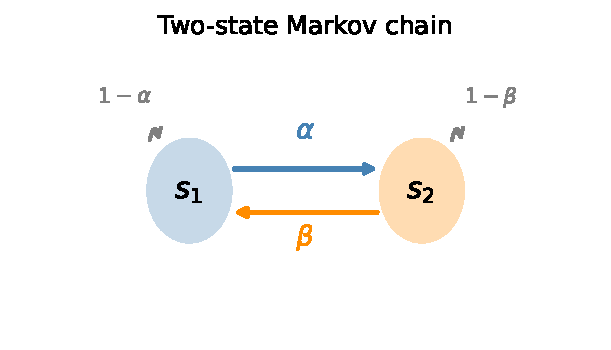
\includegraphics[width=\linewidth]{fig_two_state_chain}
  \end{column}
  \begin{column}{0.46\textwidth}
    \textbf{Two-state chain:}
    $\bfP = \begin{pmatrix}1-\alpha & \alpha \\ \beta & 1-\beta\end{pmatrix}$
    with $\alpha, \beta \in (0,1)$.

    \smallskip
    The unique stationary distribution is
    $\pi = \bigl(\tfrac{\beta}{\alpha+\beta},\, \tfrac{\alpha}{\alpha+\beta}\bigr)$.
  \end{column}
\end{columns}

\end{frame}

\begin{frame}[allowframebreaks]{6.2 Ergodic Theorem and Convergence}

The key theoretical guarantee for MCMC is the following fundamental result.

\begin{block}{Proposition 6.2.2 (Ergodic Theorem for Markov Chains)}
If $\bfP$ is \textbf{regular} (ergodic), then there exists a \textbf{unique} stationary distribution $\pi$ with all entries strictly positive, and
\[
  \bfP^n \to \bm{\Pi} \quad \text{as } n \to \infty,
\]
where $\bm{\Pi}$ is the matrix all of whose rows equal $\pi$.
\end{block}

In other words, regardless of the initial state, after a sufficiently long time the distribution of the chain converges to $\pi$.

\begin{block}{Corollary 6.2.3}
For any initial distribution $\bfmu$:
\[
  \bfmu \bfP^n \to \bfpi \quad \text{as } n \to \infty.
\]
\end{block}

\framebreak

To quantify \emph{how fast} the chain converges, we use the \textbf{total variation distance}.

\begin{block}{Total Variation Distance and Mixing Time}
For two probability vectors $\bfmu$ and $\bfv$ on $\mathcal{S}$:
\[
  \dTV(\bfmu, \bfv) = \frac{1}{2} \sum_{s \in \mathcal{S}} |\mu_s - v_s| = \max_{A \subseteq \mathcal{S}} |\mu(A) - \nu(A)|.
\]
The factor $1/2$ ensures $\dTV \in [0,1]$: when $\dTV = 0$ the distributions are identical; when $\dTV = 1$ they have disjoint supports.

The \textbf{mixing time} $\tau(\varepsilon)$ is the number of steps needed to get within $\varepsilon$ of $\pi$:
\[
  \tau(\varepsilon) = \min_{n \in \mathbb{N}} \bigl\{ \dTV(\bfmu \bfP^n, \bfpi) \le \varepsilon \bigr\}.
\]
\end{block}

Corollary 6.2.3 implies $\lim_{n \to \infty} \dTV(\bfmu \bfP^n, \bfpi) = 0$ for every $\bfmu$.

\framebreak

The following proposition explains how to simulate a Markov chain in practice.

\begin{block}{Proposition 6.2.4 (Update Function Representation)}
For any transition matrix $\bfP$ and initial distribution $\bfmu$, there exist functions $\varphi : \mathcal{S} \times [0,1] \to \mathcal{S}$ and $\psi : [0,1] \to \mathcal{S}$ such that
\[
  X_0 = \psi(U_0), \qquad X_{n+1} = \varphi(X_n,\, U_{n+1}),
\]
where $U_0, U_1, \ldots$ are i.i.d.\ $\mathcal{U}[0,1]$.
\end{block}

The function $\varphi$ is called the \textbf{update function} and $\psi$ the \textbf{initialisation function}.
A canonical construction of $\varphi$ is
\[
  \varphi(s, u) = s_k \quad \text{if } u \in \Bigl[\sum_{j<k} p_{s,s_j},\, \sum_{j \le k} p_{s,s_j}\Bigr).
\]
This representation is essential for the Coupling from the Past algorithm (Section~6.4).

\begin{alertblock}{Key Takeaway}
Every Markov chain can be driven by a stream of i.i.d.\ uniform random variables through an update function.
This means we can run \emph{multiple chains simultaneously using the same randomness}, which is the basis of the coupling idea.
\end{alertblock}

\end{frame}

\begin{frame}[allowframebreaks]{6.2 Detailed Balance and Random Walks on Graphs}

Instead of solving $\bfpi \bfP = \bfpi$ directly, the \emph{detailed balance condition} (DBC) provides a simpler sufficient condition for stationarity.

\begin{block}{Proposition 6.2.5 (Detailed Balance Condition)}
Suppose there exist strictly positive weights $(w_s)_{s \in \mathcal{S}}$ satisfying
\[
  w_s\, p_{ss'} = w_{s'}\, p_{s's} \qquad \text{for all } s, s' \in \mathcal{S}. \tag{DBC}
\]
Then $\pi_s = w_s / \sum_{s''} w_{s''}$ is a stationary distribution for $\bfP$.
\end{block}

\textbf{Proof sketch.} Setting $w_s = \pi_s$ and summing over $s$:
$\sum_s \pi_s p_{ss'} = \sum_s \pi_{s'} p_{s's} = \pi_{s'} \sum_s p_{s's} = \pi_{s'}$. $\square$

The DBC is equivalent to \textbf{time-reversibility}: if $X_0 \sim \pi$ then $(X_0, X_1, \ldots, X_n) \overset{d}{=} (X_n, X_{n-1}, \ldots, X_0)$.
A chain satisfying DBC is called \emph{reversible}.

\begin{block}{Corollary 6.2.6}
If $\bfP$ is symmetric ($p_{ss'} = p_{s's}$ for all $s,s'$), then the stationary distribution is \emph{uniform}: $\pi_s = 1/|\mathcal{S}|$.
\end{block}

\framebreak

\begin{block}{Example 6.2.7: Simple Random Walk on Graph $G = (V,E)$}
The simple random walk moves from vertex $v$ to any of its neighbours with equal probability:
\[
  q_{vv'} = \begin{cases} \tfrac{1}{\deg(v)}, & \text{if } \{v,v'\} \in E, \\ 0, & \text{otherwise.} \end{cases}
\]
Setting $w_v = \deg(v)$, we check DBC:
$w_v\, q_{vv'} = \deg(v) \cdot \tfrac{1}{\deg(v)} = 1 = \deg(v') \cdot \tfrac{1}{\deg(v')} = w_{v'} q_{v'v}$
(since for neighbors $q_{vv'} > 0$ iff $q_{v'v} > 0$).
Thus the stationary distribution is
\[
  \pi_v = \frac{\deg(v)}{\sum_{v'} \deg(v')} = \frac{\deg(v)}{2|E|}.
\]
The stationary distribution is proportional to degree; for regular graphs (all degrees equal) it is uniform.
\end{block}

\begin{block}{Example 6.2.9: Adding Self-loops for Aperiodicity}
If the graph is bipartite (e.g.\ a path graph $1-2-3-\cdots$), the simple random walk is periodic with period 2.
Adding a self-loop probability $\beta \in (0,1)$:
$q_{vv} = \beta$, $q_{vv'} = (1-\beta)/\deg(v)$ for $\{v,v'\} \in E$,
makes the chain aperiodic without changing the stationary distribution.
\end{block}

\end{frame}

% ============================================================
\section{6.3 Constructing MCMC Chains}
% ============================================================

\begin{frame}[allowframebreaks]{6.3 The MCMC Construction Problem}

We now address the central challenge: given a target distribution $\pi$ on a large or complex state space $\mathcal{S}$, how do we construct a Markov chain that has $\pi$ as its stationary distribution and is easy to simulate?

The \textbf{Markov Chain Monte Carlo} (MCMC) framework builds such a chain.
A key observation is that to check the DBC (or to compute acceptance ratios in the algorithms below), we only need to evaluate \emph{ratios} $\pi_{s'}/\pi_s$.
If $\pi_s = c \cdot \tilde{\pi}_s$ for some known $\tilde{\pi}_s$ but unknown constant $c$, the constant cancels:
\[
  \frac{\pi_{s'}}{\pi_s} = \frac{\tilde{\pi}_{s'}}{\tilde{\pi}_s}.
\]
This is why MCMC works even when the normalising constant is unknown.

\framebreak

The two canonical MCMC algorithms are:
\begin{itemize}
  \item \textbf{Metropolis-Hastings} (Section~6.3.1): propose a new state from an arbitrary ``proposal'' distribution, then accept or reject the proposal based on a ratio test that guarantees stationarity.
  \item \textbf{Gibbs sampler} (Section~6.3.2): applicable when the state space has a product structure $\mathcal{S} = C^V$; update one coordinate at a time by sampling from the exact conditional distribution of that coordinate given all others.
\end{itemize}

Both algorithms produce a Markov chain satisfying the DBC with weights $w_s = \pi_s$, hence having stationary distribution $\pi$.

\end{frame}

% ────────────────────────────────────
\subsection{6.3.1 Metropolis and Metropolis-Hastings}
% ────────────────────────────────────

\begin{frame}[allowframebreaks]{6.3.1 The Metropolis Algorithm}

\textbf{Setting.} We are given a target distribution $\pi$ on $\mathcal{S}$ and a \emph{symmetric}, regular transition matrix $\bfQ = (q_{ss'})$ called the \emph{candidate-generating matrix} or \emph{proposal matrix}.
From the current state $s$, we propose moving to $s' \sim \mathbf{q}_s$.
The proposal is accepted with probability $\min(1, \pi_{s'}/\pi_s)$; otherwise we stay at $s$.

\begin{block}{The Metropolis Transition Matrix}
The resulting transition matrix $\bfP$ has entries
\[
  p_{ss'} = \begin{cases}
    q_{ss'} \min\!\left(1, \dfrac{\pi_{s'}}{\pi_s}\right), & s \neq s', \\[6pt]
    1 - \displaystyle\sum_{k \neq s} q_{sk} \min\!\left(1, \dfrac{\pi_k}{\pi_s}\right), & s = s'.
  \end{cases}
\]
\end{block}

\begin{block}{Algorithm 42 (Metropolis, one step)}
\textbf{Given:} Current state $Y_k = s$; symmetric proposal $\bfQ$; target $\pi$.
\begin{enumerate}
  \item Sample proposed state $X \sim \mathbf{q}_s = (q_{s,s_1}, \ldots, q_{s,s_N})$.
  \item Compute acceptance probability $\alpha = \min\!\left(1,\, \pi_X / \pi_s\right)$.
  \item Draw $U \sim \mathcal{U}[0,1]$ independently of $X$.
  \item If $U \le \alpha$: \textbf{accept} and set $Y_{k+1} = X$; otherwise $Y_{k+1} = Y_k$.
\end{enumerate}
\end{block}

\framebreak

\textbf{Why does this work?} We verify the DBC with $w_s = \pi_s$.
For $s \neq s'$ (assuming $q_{ss'} > 0$):
\begin{align*}
  \pi_s \, p_{ss'} &= \pi_s \, q_{ss'} \min(1, \pi_{s'}/\pi_s) = q_{ss'} \min(\pi_s, \pi_{s'}).
\end{align*}
By symmetry of $\bfQ$ ($q_{ss'} = q_{s's}$) and symmetry of $\min$:
\[
  \pi_{s'} \, p_{s's} = q_{s's} \min(\pi_{s'}, \pi_s) = \pi_s \, p_{ss'}. \checkmark
\]

\begin{block}{Proposition 6.3.1 (Metropolis)}
If $\bfQ$ is symmetric and regular, then the Metropolis transition matrix $\bfP$ is regular with stationary distribution $\pi$.
\end{block}

\begin{exampleblock}{Worked Example: Two-State Metropolis}
Let $\mathcal{S} = \{0,1\}$, $\pi_0 = 0.3$, $\pi_1 = 0.7$, and $\bfQ = \begin{pmatrix}0 & 1\\ 1 & 0\end{pmatrix}$ (always propose the other state).

From state 0: accept probability $= \min(1, 0.7/0.3) = 1$, so $p_{01} = 1$.

From state 1: accept probability $= \min(1, 0.3/0.7) = 3/7$, so $p_{10} = 3/7$, $p_{11} = 4/7$.

Stationary check: $\pi_0 \cdot 1 = 0.3 = (3/7) \cdot 0.7 = \pi_1 \cdot p_{10}$. The DBC holds.
\end{exampleblock}

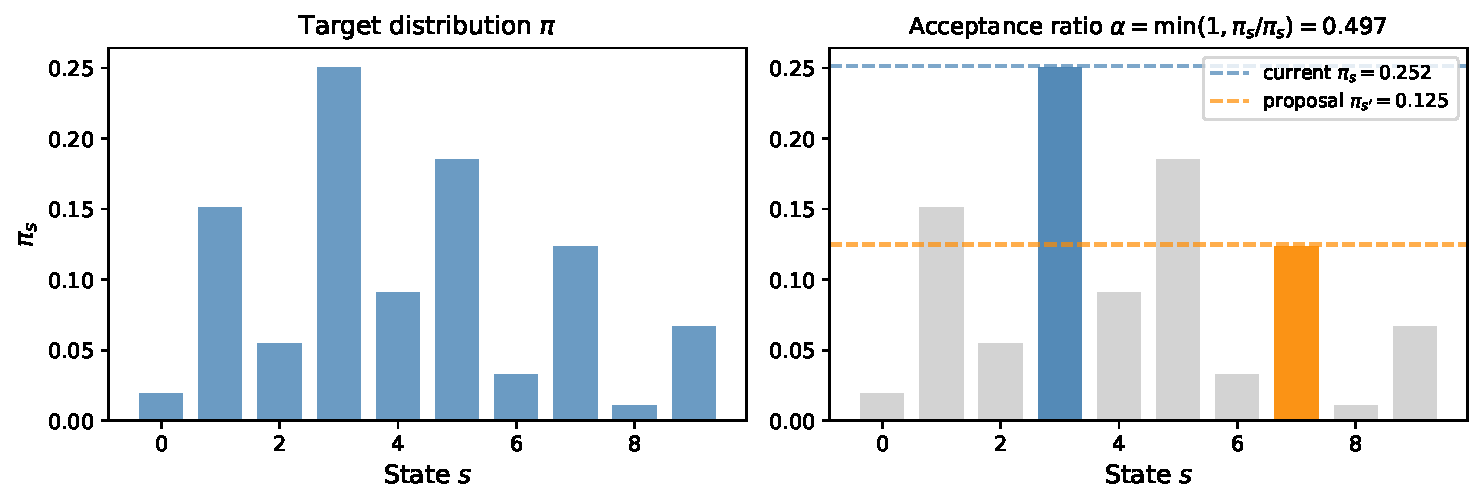
\includegraphics[width=0.75\linewidth]{fig_metropolis_acceptance}

\end{frame}

\begin{frame}[allowframebreaks]{6.3.1 Metropolis-Hastings: Asymmetric Proposals}

The Metropolis algorithm requires a symmetric proposal $\bfQ$.
The \textbf{Metropolis-Hastings} (MH) algorithm removes this restriction, making it applicable to any regular proposal matrix.

\begin{block}{Algorithm 43 (Metropolis-Hastings, one step)}
\textbf{Given:} Current state $Y_k = s$; regular proposal matrix $\bfQ$; target $\pi$.
\begin{enumerate}
  \item Sample proposed state $X \sim \mathbf{q}_s$.
  \item Compute the \textbf{Hastings acceptance ratio}:
        $\displaystyle\alpha_{sX} = \min\!\left(1,\, \frac{\pi_X \, q_{Xs}}{\pi_s \, q_{sX}}\right)$.
  \item Draw $U \sim \mathcal{U}[0,1]$. If $U \le \alpha_{sX}$: set $Y_{k+1} = X$; else $Y_{k+1} = Y_k$.
\end{enumerate}
\end{block}

The factor $\pi_X q_{Xs} / (\pi_s q_{sX})$ corrects for the asymmetry in the proposal: if $\bfQ$ tends to over-propose moves from $s$ to $s'$ (i.e.\ $q_{ss'} \gg q_{s's}$), the correction factor downweights acceptance.

\begin{block}{Proposition 6.3.2 (Metropolis-Hastings)}
Let $\bfQ$ be regular with $q_{ss'} > 0 \Leftrightarrow q_{s's} > 0$. Then the MH transition matrix
\[
  p_{ss'} = q_{ss'}\, \alpha_{ss'} \quad (s \neq s'), \qquad \alpha_{ss'} = \min\!\left(1,\, \frac{\pi_{s'}\,q_{s's}}{\pi_s\,q_{ss'}}\right),
\]
is regular with stationary distribution $\pi$.
\end{block}

\textbf{Proof.} For $s \neq s'$:
\[
  \pi_s q_{ss'} \min\!\Bigl(1, \frac{\pi_{s'}q_{s's}}{\pi_s q_{ss'}}\Bigr) = \min(\pi_s q_{ss'},\, \pi_{s'} q_{s's}) = \pi_{s'} q_{s's} \min\!\Bigl(1, \frac{\pi_s q_{ss'}}{\pi_{s'} q_{s's}}\Bigr). \quad \square
\]

\framebreak

\textbf{Special case: Random Walk MH on a graph.}
On a connected graph $G = (V,E)$, take $q_{vv'} = 1/K$ if $v' \in \mathcal{N}(v)$ (and $q_{vv} = 1 - \deg(v)/K$ for a self-loop, with $K \ge \Delta = \max\deg$).
To sample from a target $\pi_v = b_v/B$ (with $B = \sum b_v$ unknown), the acceptance ratio becomes:
\[
  \alpha_{vv'} = \min\!\left(1,\, \frac{\pi_{v'}/K}{\pi_v/K}\right) = \min\!\left(1,\, \frac{b_{v'}}{b_v}\right).
\]
The normalising constant $B$ cancels completely.

\begin{alertblock}{Key Insight: Normalising Constant Cancels}
In any MH algorithm, the target $\pi$ enters only through ratios $\pi_{s'}/\pi_s$.
If $\pi_s = \tilde\pi_s / Z$ for unknown $Z$, then $\pi_{s'}/\pi_s = \tilde\pi_{s'}/\tilde\pi_s$.
This is the single most important practical advantage of MCMC over direct sampling.
\end{alertblock}

\end{frame}

\begin{frame}[fragile]{6.3.1 Metropolis-Hastings: Python Implementation}
\begin{lstlisting}[style=python]
import numpy as np

def metropolis_hastings(log_pi, proposal, x0, n_steps):
    """
    Generic Metropolis-Hastings sampler.
    log_pi  : callable, log of (unnormalized) target density
    proposal: callable, proposal(x) -> (x_new, log_q_ratio)
              where log_q_ratio = log q(x_new->x) - log q(x->x_new)
    x0      : initial state
    n_steps : number of steps
    """
    samples = [x0]
    x = x0
    n_accept = 0
    for _ in range(n_steps):
        x_new, log_q_ratio = proposal(x)
        # MH acceptance ratio (in log space for numerical stability)
        log_alpha = (log_pi(x_new) - log_pi(x)) + log_q_ratio
        if np.log(np.random.rand()) < log_alpha:
            x = x_new
            n_accept += 1
        samples.append(x)
    print(f"Acceptance rate: {n_accept/n_steps:.1%}")
    return np.array(samples)

# Example: mixture of two Gaussians (unknown normalizing constant)
def log_pi_mix(x):
    return np.log(0.4*np.exp(-0.5*(x+2)**2) + 0.6*np.exp(-0.5*(x-3)**2/4))

# Symmetric random-walk proposal: q_ratio = 0
def rw_proposal(x, sigma=1.5):
    x_new = x + np.random.normal(0, sigma)
    return x_new, 0.0  # symmetric => log q(x_new->x) = log q(x->x_new)

np.random.seed(42)
chain = metropolis_hastings(log_pi_mix, rw_proposal, x0=0.0, n_steps=5000)
I_hat = chain[500:].mean()   # discard first 500 as burn-in
print(f"E[X] estimate: {I_hat:.4f}")
\end{lstlisting}
\end{frame}

\begin{frame}{6.3.1 MH Trace: Convergence in Practice}

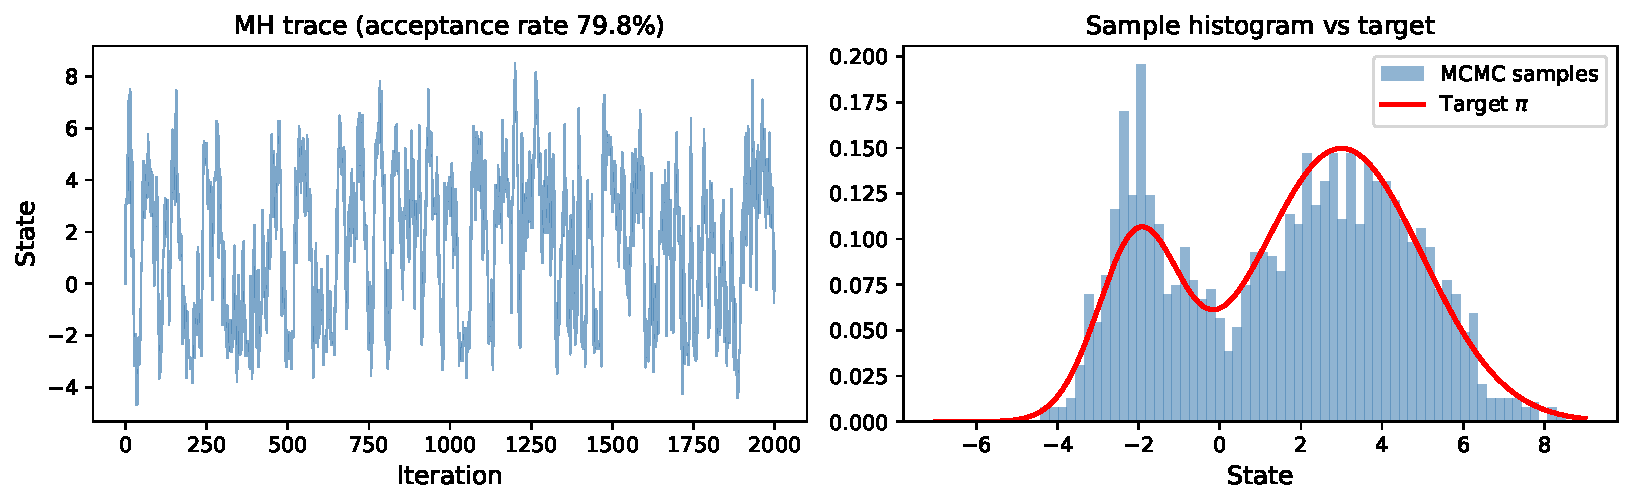
\includegraphics[width=\linewidth]{fig_mh_trace}

Three phases are visible in a typical MCMC run.
\begin{enumerate}
  \item \textbf{Burn-in}: the chain has not yet reached its stationary distribution, so samples are biased.
  \item \textbf{Mixing}: the chain traverses the support of $\pi$ and samples become representative.
  \item \textbf{Estimation}: we average $f(X_j)$ over the post-burn-in samples.
\end{enumerate}

The choice of proposal step size $\sigma$ is crucial: too small leads to slow exploration (high acceptance, small moves); too large leads to many rejections (low acceptance, chain stays put).
For a random walk proposal in $\mathbb{R}^d$, the theoretically optimal acceptance rate is approximately 23\%.

\begin{alertblock}{Key Takeaway}
The burn-in period is discarded; the remaining samples form a (correlated) sequence from $\approx \pi$.
The convergence diagnostic is monitoring $\hat{Y}_R$ as a running average: once it stabilises, the chain has mixed.
\end{alertblock}

\end{frame}

% ────────────────────────────────────
\subsection{6.3.2 Gibbs Sampler}
% ────────────────────────────────────

\begin{frame}[allowframebreaks]{6.3.2 The Gibbs Sampler: Setup and Motivation}

The Gibbs sampler applies when the state space has a \emph{product structure} $\mathcal{S} = C^V$, where $V$ is a finite set of vertices (coordinates) and $C = \{1, \ldots, r\}$ is a finite alphabet.
A \emph{configuration} $\xi \in \mathcal{S}$ is a function $\xi : V \to C$ assigning a value $\xi(v) \in C$ to each vertex $v \in V$.

Many important models have this structure, including spin systems in statistical physics and Markov random fields in machine learning.

The Gibbs sampler updates one coordinate at a time, sampling it from its \emph{full conditional distribution} given all other coordinates.
This is particularly natural for \textbf{Gibbs distributions}:
\[
  \pi_\xi = \frac{1}{z(T)}\, e^{-H(\xi)/T},
\]
where $H : \mathcal{S} \to \mathbb{R}$ is an \emph{energy function}, $T > 0$ is the \emph{temperature}, and $z(T) = \sum_{\xi \in \mathcal{S}} e^{-H(\xi)/T}$ is the partition function (normalising constant).

\framebreak

\begin{block}{Full Conditional Distribution}
Given a configuration $\xi \in \mathcal{S}$ and a vertex $v \in V$, we write $\xi_{-v}$ for the restriction of $\xi$ to all vertices except $v$.
The \textbf{full conditional distribution} of coordinate $v$ given all others is
\[
  p_{\xi,v}(c) = \PP(Z(v) = c \mid Z_{-v} = \xi_{-v}), \quad c \in C,
\]
where $Z \sim \pi$. This is the conditional distribution of the value at $v$, given that all other vertices take their current values according to $\xi$.
\end{block}

\begin{block}{Algorithm 44 (Gibbs Sampler, one step)}
\textbf{Given:} Current configuration $X_k = \xi$; target $\pi$.
\begin{enumerate}
  \item Choose a vertex $v \in V$ uniformly at random.
  \item For each $c \in C$, compute the weight $p_{\xi,v}(c)$ proportional to $\pi_{\xi(v \to c)}$, where $\xi(v \to c)$ denotes $\xi$ with the value at $v$ changed to $c$.
  \item Sample $c^* \sim p_{\xi,v}(\cdot)$ (the full conditional).
  \item Set $X_{k+1}(v) = c^*$ and $X_{k+1}(w) = \xi(w)$ for $w \neq v$.
\end{enumerate}
\end{block}

\framebreak

The update function for the Gibbs sampler, using $X_{n+1} = \varphi(X_n, W_{n+1}, U_{n+1})$ where $W_{n+1}$ is the randomly chosen vertex and $U_{n+1} \in [0,1]$, is
\[
  \varphi(\xi, v, u) = \xi(v \to c) \quad \text{if } u \in \Bigl[\sum_{c' < c} p_{\xi,v}(c'),\; \sum_{c' \le c} p_{\xi,v}(c')\Bigr).
\]

\begin{block}{Proposition 6.3.5 (Gibbs Sampler Correctness)}
If the Gibbs sampler chain is ergodic, its stationary distribution is $\pi$.
\end{block}

\textbf{Proof.} We verify DBC for any two configurations $\xi, \xi' \in \mathcal{S}$ that differ at exactly one vertex $v$:
\[
  \pi_\xi \cdot p_{\xi\xi'} = \pi_\xi \cdot \frac{1}{|V|} p_{\xi,v}(\xi'(v)) = \frac{\pi_\xi \pi_{\xi'}}{|V| \sum_{c} \pi_{\xi(v \to c)}}.
\]
This is symmetric in $\xi$ and $\xi'$, confirming DBC. $\square$

\begin{exampleblock}{Note on Ergodicity}
The Gibbs sampler can fail to be ergodic (e.g., be reducible or periodic).
Regularity must be checked for each specific model.
\end{exampleblock}

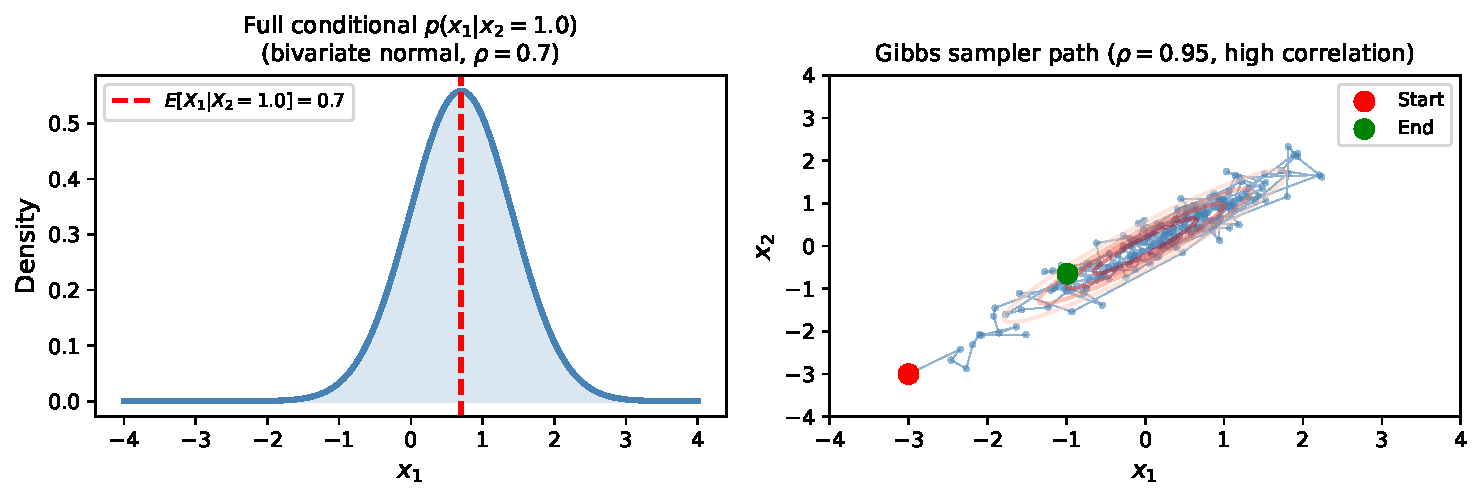
\includegraphics[width=0.80\linewidth]{fig_gibbs_full_conditional}

\end{frame}

% ────────────────────────────────────
\subsubsection{Graph Coloring}
% ────────────────────────────────────

\begin{frame}[allowframebreaks]{6.3.2.1 Graph Coloring}

\textbf{Problem.} Given a graph $G = (V,E)$ and a colour set $C = \{1, \ldots, r\}$, a \emph{proper $r$-colouring} is an assignment $\xi : V \to C$ such that no two adjacent vertices share the same colour, i.e.\ $\xi(v) \neq \xi(v')$ for all $\{v,v'\} \in E$.
Let $\Lambda$ be the set of all proper colourings and $z_G = |\Lambda|$.

\begin{block}{Target Distribution: Uniform over Proper Colourings}
\[
  \pi_\xi = \frac{1}{z_G}\, \mathbf{1}(\xi \in \Lambda).
\]
\end{block}

Computing $z_G$ exactly is \#P-complete in general, but sampling from $\pi$ is tractable via Gibbs sampling when $r$ is sufficiently large.

\framebreak

\textbf{Gibbs sampler for graph colouring (Algorithm 45).}
Given current colouring $\xi$, pick vertex $v \in V$ uniformly at random.
Let $\mathcal{C}_{\xi,v} = \{\xi(w) : w \in \mathcal{N}(v)\}$ be the set of colours used by $v$'s neighbours.
The full conditional distribution is uniform over all \emph{available} colours:
\[
  p_{\xi,v}(c) = \begin{cases}
    0, & c \in \mathcal{C}_{\xi,v}, \\
    \dfrac{1}{r - |\mathcal{C}_{\xi,v}|}, & c \in C \setminus \mathcal{C}_{\xi,v}.
  \end{cases}
\]
Pick $c^*$ uniformly from $C \setminus \mathcal{C}_{\xi,v}$ and set $\xi(v) \leftarrow c^*$.

\begin{columns}[T]
  \begin{column}{0.5\textwidth}
    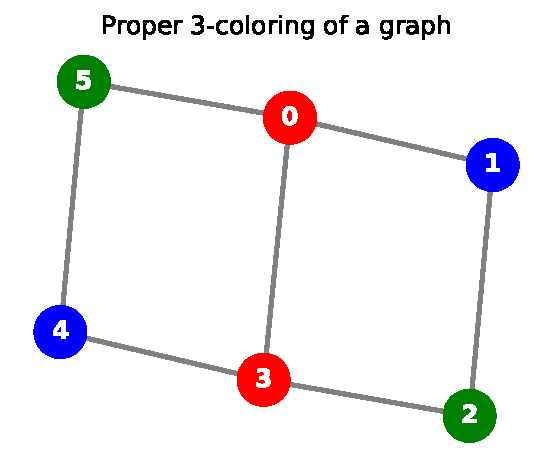
\includegraphics[width=\linewidth]{fig_graph_coloring}
  \end{column}
  \begin{column}{0.46\textwidth}
    The Gibbs sampler requires $r \ge \Delta + 1$ to ensure there is always at least one available colour (so the chain is well-defined from any proper colouring).

    \smallskip
    \textbf{Metropolis alternative (Algorithm 46):} choose $v \in V$ and $c \in C$ uniformly; accept the new colouring $\xi(v \leftarrow c)$ if it is still proper.
    The acceptance ratio is $\pi_{\xi'}/\pi_\xi = 1$ (if feasible) or $0$ (if not).
  \end{column}
\end{columns}

\framebreak

\begin{block}{Rapid Mixing (Lemma 6.5.15)}
If $r \ge 2\Delta + 1$ (where $\Delta = \max_{v \in V} \deg(v)$), the Metropolis chain on colourings is \textbf{rapidly mixing} with mixing time
\[
  \tau(\kappa) \le \frac{r}{r - 2\Delta}\, M\, \ln\!\left(\frac{M}{\kappa}\right), \quad M = |V|.
\]
This bound is polynomial in $M$ and $\ln(1/\kappa)$, meaning the chain reaches stationarity efficiently even for large graphs.
\end{block}

\begin{alertblock}{Remark on Ergodicity}
If $r = \Delta$ exactly, the chain may be periodic or reducible.
For example, on the complete graph $K_3$ with $r = 3$ colours, once a valid 3-colouring is reached, no vertex can change its colour without creating a conflict, so the chain is absorbing (not ergodic).
Always verify $r > \Delta$ to ensure ergodicity.
\end{alertblock}

\end{frame}

% ────────────────────────────────────
\subsubsection{Hard-core Model}
% ────────────────────────────────────

\begin{frame}[allowframebreaks]{6.3.2.2 Hard-core Model}

\textbf{Problem.} Given a graph $G = (V,E)$ and a parameter $\lambda > 0$, each vertex is either \emph{occupied} ($\xi(v) = 1$) or \emph{empty} ($\xi(v) = 0$).
A configuration $\xi \in \{0,1\}^V$ is \emph{feasible} (an \emph{independent set}) if no two occupied vertices are adjacent: $\xi(v) = \xi(w) = 1 \Rightarrow \{v,w\} \notin E$.

\begin{block}{Generalised Hard-core Distribution}
\[
  \pi_\xi = \frac{\lambda^{m(\xi)}}{z_{G,\lambda}}\, \mathbf{1}(\xi \in \Lambda),
  \quad z_{G,\lambda} = \sum_{\xi \in \Lambda} \lambda^{m(\xi)},
\]
where $m(\xi) = \sum_{v \in V} \xi(v)$ is the number of occupied vertices and $\Lambda$ is the set of all independent sets.
For $\lambda = 1$ this reduces to the uniform distribution over $\Lambda$.
For $\lambda > 1$, configurations with more particles are favoured.
\end{block}

\framebreak

\textbf{Full conditional for the hard-core model.}
Given configuration $\xi$ and vertex $v$, there are two cases:
\begin{itemize}
  \item If any neighbour $w \in \mathcal{N}_G(v)$ has $\xi(w) = 1$: the vertex $v$ cannot be occupied, so $p_{\xi,v}(1) = 0$ and $p_{\xi,v}(0) = 1$.
  \item If all neighbours of $v$ are empty ($\xi(w) = 0$ for all $w \in \mathcal{N}_G(v)$): then
        \[
          p_{\xi,v}(1) = \frac{\lambda}{\lambda + 1}, \quad p_{\xi,v}(0) = \frac{1}{\lambda + 1}.
        \]
\end{itemize}

\begin{block}{Algorithm 47 (Gibbs Sampler for Hard-core Model)}
\textbf{Given:} Graph $G = (V,E)$, parameter $\lambda > 0$.
\begin{enumerate}
  \item Choose $v \in V$ uniformly at random and flip a biased coin: heads with probability $\lambda/(\lambda+1)$.
  \item If any neighbour of $v$ is occupied: set $\xi(v) = 0$ regardless.
  \item If all neighbours are empty: set $\xi(v) = 1$ on heads, $\xi(v) = 0$ on tails.
\end{enumerate}
\end{block}

\begin{columns}[T]
  \begin{column}{0.52\textwidth}
    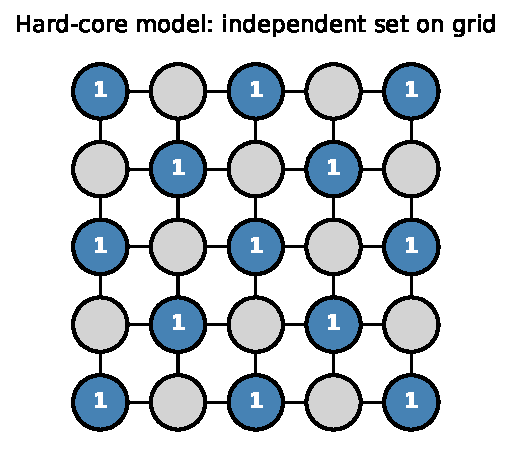
\includegraphics[width=\linewidth]{fig_hardcore_grid}
  \end{column}
  \begin{column}{0.44\textwidth}
    The figure shows typical configurations of the hard-core model on a grid graph for different values of $\lambda$.
    For large $\lambda$, configurations concentrate on maximum independent sets (checkerboard patterns on a grid).
  \end{column}
\end{columns}

\end{frame}

% ────────────────────────────────────
\subsubsection{Ising Model}
% ────────────────────────────────────

\begin{frame}[allowframebreaks]{6.3.2.4 Ising Model}

The Ising model is one of the most studied models in statistical physics and serves as a canonical example for MCMC.

\textbf{Setup.} Consider a graph $G = (V,E)$ (typically a 2D grid) where each vertex $v \in V$ carries a \emph{spin} $\xi(v) \in \{-1, +1\}$.

\begin{block}{Ising Distribution}
The energy of a configuration $\xi \in \{-1,+1\}^V$ is
\[
  H(\xi) = -\sum_{\{v,v'\} \in E} \xi(v)\,\xi(v').
\]
Note that $H(\xi)$ is low when neighbouring spins align.
The Ising distribution is the Gibbs measure with inverse temperature $\beta \in \mathbb{R}$:
\[
  \pi_\xi = \frac{1}{z_\beta}\,\exp(\beta \sum_{\{v,v'\} \in E} \xi(v)\,\xi(v')) = \frac{e^{-\beta H(\xi)}}{z_\beta}.
\]
When $\beta > 0$ (ferromagnet), aligned configurations have higher probability. When $\beta < 0$ (anti-ferromagnet), alternating configurations are favoured.
\end{block}

\framebreak

\textbf{Full conditional for the Ising model.}
Let $m_+(v,\xi) = \#\{w \in \mathcal{N}(v) : \xi(w) = +1\}$ and $m_-(v,\xi) = \#\{w \in \mathcal{N}(v) : \xi(w) = -1\}$.
Then
\[
  \PP(Z(v) = +1 \mid Z_{-v} = \xi_{-v}) = \alpha(\xi, v), \quad \alpha(\xi,v) = \frac{1}{1 + e^{-2\beta(m_+(v,\xi) - m_-(v,\xi))}}.
\]
Derivation: the energy difference between $\xi(v) = +1$ and $\xi(v) = -1$ (with all others fixed) is $-2\beta \sum_{w \in \mathcal{N}(v)} \xi(w)$, which simplifies to $-2\beta(m_+ - m_-)$.

\begin{block}{Algorithm 48 (Gibbs Sampler for Ising Model)}
\textbf{Given:} Graph $G = (V,E)$, parameter $\beta$.
\begin{enumerate}
  \item Choose $v \in V$ uniformly at random; draw $U \sim \mathcal{U}[0,1]$.
  \item Compute $\alpha(\xi, v) = 1/(1 + \exp(-2\beta(m_+(v,\xi) - m_-(v,\xi))))$.
  \item Set $\xi(v) = +1$ if $U < \alpha(\xi,v)$; else $\xi(v) = -1$.
\end{enumerate}
\end{block}

\begin{columns}[T]
  \begin{column}{0.52\textwidth}
    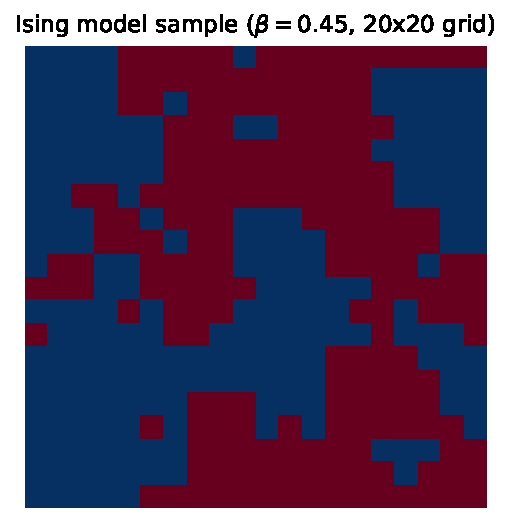
\includegraphics[width=\linewidth]{fig_ising_sample}
  \end{column}
  \begin{column}{0.44\textwidth}
    \textbf{Phase transition.} On the 2D integer lattice, the 2D Ising model undergoes a phase transition at the \emph{critical temperature}:
    \[
      \beta_c = \tfrac{1}{2}\ln(1 + \sqrt{2}) \approx 0.4407.
    \]
    Below $\beta_c$: no long-range order (disordered phase). Above $\beta_c$: spontaneous magnetisation (ordered phase).
  \end{column}
\end{columns}

\end{frame}

\begin{frame}[fragile]{6.3.2.4 Ising Model: Python Implementation}
\begin{lstlisting}[style=python]
import numpy as np
import matplotlib.pyplot as plt

def ising_gibbs(n, beta, n_steps=100000, seed=0):
    """
    Gibbs sampler for Ising model on n x n periodic grid.
    n     : grid size
    beta  : inverse temperature (>0 ferromagnet, <0 antiferromagnet)
    """
    np.random.seed(seed)
    config = np.random.choice([-1, 1], size=(n, n))

    for step in range(n_steps):
        i, j = np.random.randint(0, n, 2)
        # Sum of four neighboring spins (periodic boundary conditions)
        nbr_sum = (config[(i-1)%n, j] + config[(i+1)%n, j]
                 + config[i, (j-1)%n] + config[i, (j+1)%n])
        # Full conditional: P(spin = +1 | neighbors)
        # alpha = 1 / (1 + exp(-2*beta*nbr_sum))
        h = beta * nbr_sum
        prob_plus = np.exp(h) / (np.exp(h) + np.exp(-h))
        config[i, j] = 1 if np.random.rand() < prob_plus else -1

    return config

# Run near the critical temperature
config = ising_gibbs(n=20, beta=0.44, n_steps=200000)
magnetization = config.mean()
print(f"Magnetization: {magnetization:.4f}")
# Expected: near 0 (disordered) or near +-1 (ordered)
# depending on initial configuration and finite-size effects
\end{lstlisting}

The critical temperature $\beta_c \approx 0.4407$ is computed from Onsager's exact solution of the 2D Ising model.
Near $\beta_c$ the chain mixes very slowly (critical slowing down), so special algorithms (e.g.\ cluster algorithms) are needed.
\end{frame}

% ============================================================
\section{6.4 Perfect Simulation}
% ============================================================

\begin{frame}[allowframebreaks]{6.4 Perfect Simulation: Motivation and CFTP}

\textbf{The problem with standard MCMC.}
The Markov chain $(X_n)$ only \emph{approximates} $\pi$ after $n$ steps; we never know exactly how close $\bfmu \bfP^n$ is to $\bfpi$ without knowing the mixing time.
In practice, determining an adequate burn-in requires additional analysis or heuristics.

\begin{block}{Perfect Simulation (Definition)}
A \textbf{perfect simulation} algorithm generates a sample that has distribution \emph{exactly} $\pi$, in finite (random) time, without knowing the mixing time.
\end{block}

The key idea, due to Propp and Wilson (1996), is \textbf{Coupling from the Past (CFTP)}.

\framebreak

\textbf{The CFTP idea.}
Instead of running the chain forward from a single initial state, we run it \emph{backward} from time $-N$ to time $0$, starting simultaneously from \emph{all} possible initial states, using the \emph{same} sequence of random variables.
If all chains end up in the same state $Z$ at time $0$, then $Z \sim \pi$ exactly.

Why backward? If we run chains from time $-N$ to time $0$ using the same $U_{-N}, \ldots, U_{-1}, U_0$, and they all coalesce at time $0$ to some state $Z$, then $Z$ is the same regardless of where the chain started at $-N$.
Since the ergodic theorem guarantees every initial state eventually produces $Z \sim \pi$, the output of CFTP is exactly $\pi$-distributed.

\begin{block}{Algorithm 49 (CFTP --- General Version)}
\textbf{Require:} State space $\mathcal{S}$, ergodic chain $(X_n)$ with update rule $\varphi$.
\begin{enumerate}
  \item Set $n = 1$.
  \item For each $s \in \mathcal{S}$, simulate the chain $X^s$ starting from state $s$ at time $-N_n$ using the \emph{same} i.i.d.\ $U_i$, $i = -N_n, \ldots, 0$.
  \item If all chains end at the same state at time 0: output that state and stop.
  \item Else set $n = n+1$, double $N_n$, and reuse previously generated $U_i$ (extend backward).
\end{enumerate}
\end{block}

\framebreak

Running Algorithm 49 naively requires simulating $|\mathcal{S}|$ chains, which is prohibitive for large $\mathcal{S}$.
The key efficiency gain comes from \emph{monotone update functions}.

\begin{block}{Definition 6.4.3 (Realizable Monotone Chain)}
A Markov chain with update function $\varphi$ is \textbf{realizable monotone} w.r.t.\ a partial order $\preceq$ on $\mathcal{S}$ if
\[
  s \preceq s' \implies \varphi(s, u) \preceq \varphi(s', u) \quad \text{for all } u \in [0,1].
\]
\end{block}

If the chain is realizable monotone and we track only the \emph{minimum} chain (starting from $s_{\min}$) and the \emph{maximum} chain (starting from $s_{\max}$), then by the sandwich property
$s_{\min} \preceq s \preceq s_{\max}$ implies
$\varphi(s_{\min},u) \preceq \varphi(s,u) \preceq \varphi(s_{\max},u)$
for all $u$.
Thus, if the min and max chains coalesce, all chains have coalesced.

\begin{block}{Algorithm 50 (Efficient CFTP for Monotone Chains)}
Only run \emph{two} chains: one starting from $s_{\min}$ and one from $s_{\max}$.
When they coalesce at time 0, the common value is output.
\end{block}

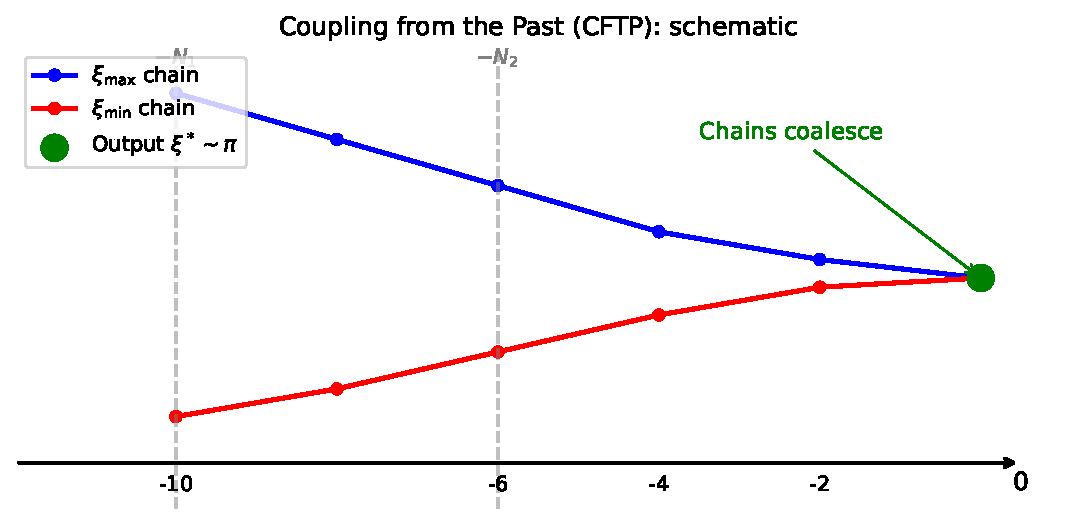
\includegraphics[width=0.85\linewidth]{fig_cftp_schematic}

\framebreak

\begin{block}{Theorem 6.4.2 (CFTP Correctness)}
Suppose $\tau_{\mathrm{cftp}}$ is finite with probability 1.
Then the output of Algorithm 49 has distribution exactly $\pi$.
\end{block}

\textbf{Proof sketch.}
For any $i > 0$, the chain $X_i^0(s) = \PP(X_i^0 = s') = \pi_{s'}$ by the ergodic theorem.
When the chain is started at $-N_j$ with $-N_j \le \tau_{\mathrm{cftp}}$, all paths coalesce:
$X_0^{-N_j}(s) = X_0^{\tau_{\mathrm{cftp}}}(s)$ for all $s$.
The latter is distributed as $\pi$ by the ergodic theorem. $\square$

\begin{block}{Proposition 6.4.5 (CFTP Terminates)}
If the chain is realizable monotone with an ergodic update function, Algorithm 50 terminates with probability 1.
\end{block}

\end{frame}

\begin{frame}[allowframebreaks]{6.4 Monotone and Anti-monotone Distributions}

\begin{block}{Definition 6.4.9 (Monotone Distribution)}
A distribution $\pi$ on $\mathcal{S} = C^V$ is \textbf{monotone} w.r.t.\ the coordinate-wise order $\preceq$ if for all $\xi \preceq \xi'$ and all $v \in V$ with $\pi_{\xi_{-v}} > 0$ and $\pi_{\xi'_{-v}} > 0$:
\[
  P(Z(v) \le c \mid Z_{-v} = \xi_{-v}) \ge P(Z(v) \le c \mid Z_{-v} = \xi'_{-v}) \quad \text{for all } c \in C.
\]
Intuitively: lower configurations make lower values of $\xi(v)$ more likely.
\end{block}

\begin{block}{Lemma 6.4.10}
If $\pi$ is monotone, then the Gibbs update function \eqref{6.3.10} is a monotone update function.
Therefore the Gibbs chain has a realizable monotone update, and Algorithm 50 applies.
\end{block}

\textbf{Example 6.4.12 (Generalised Hard-core Model).}
The generalised hard-core distribution with $\lambda > 0$ is monotone: if $\xi \preceq \xi'$ (fewer particles), the probability of adding a particle at $v$ is at least as large in $\xi$ as in $\xi'$ (fewer occupied neighbours block $v$ in $\xi$).
Wait --- actually the distribution is \emph{anti-monotone}: more particles nearby \emph{prevents} occupation of $v$.

\framebreak

\begin{block}{Definition 6.4.11 (Anti-monotone Distribution)}
A distribution $\pi$ on $\mathcal{S} = C^V$ is \textbf{anti-monotone} if for $\xi \preceq \xi'$:
\[
  P(Z(v) \le c \mid Z_{-v} = \xi_{-v}) \le P(Z(v) \le c \mid Z_{-v} = \xi'_{-v}).
\]
Higher surrounding configurations make lower values at $v$ more likely.
\end{block}

\textbf{Example 6.4.13: Ising model.}
For $\beta > 0$ (ferromagnet): $\alpha(\xi,v) = P(Z(v) = +1 | Z_{-v} = \xi_{-v})$ is \emph{increasing} in $\xi$ (more $+1$ neighbours means higher probability of $+1$ at $v$) --- the distribution is \emph{monotone}.
For $\beta < 0$ (anti-ferromagnet): $\alpha(\xi,v)$ is \emph{decreasing} in $\xi$ --- the distribution is \emph{anti-monotone}.

For anti-monotone distributions, the efficient CFTP must track a \emph{bivariate} chain $(\xi_{\min}, \xi_{\max})$ with a modified update that swaps the roles of min and max at each step.

\begin{block}{Proposition 6.4.17}
If $\pi$ is anti-monotone (and either $\pi_{\xi_{\min}} > 0$ or $\pi_{\xi_{\max}} > 0$), then the modified CFTP Algorithm 51 terminates with probability 1 and outputs a sample from $\pi$ exactly.
\end{block}

\end{frame}

\begin{frame}[fragile]{6.4 CFTP: Python Sketch for Hard-core Model}
\begin{lstlisting}[style=python]
import numpy as np

def cftp_hardcore(G, lam, max_doublings=20, seed=0):
    """
    CFTP (monotone version) for hard-core model.
    G   : dict {vertex: [neighbor_list]}
    lam : activity parameter lambda > 0
    Returns an exact sample from the hard-core distribution.
    """
    np.random.seed(seed)
    vertices = list(G.keys())
    n = len(vertices)
    prob_occ = lam / (1 + lam)  # P(occupy | all neighbors empty)

    for doubling in range(max_doublings):
        N = 2 ** doubling  # number of backward steps
        # Pre-generate: which vertex to update and acceptance coin
        vtx_idx = np.random.randint(0, n, size=N)
        coins   = np.random.rand(N)

        # Min chain: start from all-empty (xi = 0 everywhere)
        xi_min = {v: 0 for v in vertices}
        # Max chain: start from all-occupied if feasible, else largest IS
        xi_max = {v: 1 for v in vertices}  # may not be feasible, OK to start

        for k in range(N):
            v = vertices[vtx_idx[k]]
            u = coins[k]
            for xi in [xi_min, xi_max]:
                nbr_occupied = any(xi[w] for w in G[v])
                if nbr_occupied:
                    xi[v] = 0
                else:
                    xi[v] = 1 if u < prob_occ else 0

        if xi_min == xi_max:
            return xi_min  # exact sample from pi
    return xi_min  # fallback (increase max_doublings if needed)

# Example: path graph on 6 vertices
G_path = {0:[1], 1:[0,2], 2:[1,3], 3:[2,4], 4:[3,5], 5:[4]}
sample = cftp_hardcore(G_path, lam=2.0)
print("CFTP sample:", {v: sample[v] for v in sorted(sample)})
# On a path, adjacent vertices cannot both be 1
\end{lstlisting}
\end{frame}

% ============================================================
\section{6.5 Approximate Counting}
% ============================================================

\begin{frame}[allowframebreaks]{6.5 Approximate Counting: The Problem}

Many combinatorial problems ask: \emph{how many} feasible configurations exist?
For example:
\begin{itemize}
  \item How many proper $r$-colourings does a graph $G$ have? (Answer: $z_G = |\Lambda|$ for the uniform colourings distribution.)
  \item How many independent sets are in $G$?
  \item How many solutions does a 0-1 knapsack problem have?
\end{itemize}

Computing $z_G$ exactly is \#P-complete for most such problems.
However, we can approximate it efficiently using MCMC.

\begin{block}{Definition: $(\varepsilon, \delta)$-Approximation Scheme (FPRASC)}
An estimator $\hat{z}_G$ is a \textbf{fully polynomial randomised approximation scheme} (FPRASC) if
\[
  \PP\bigl(|\hat{z}_G - z_G| > \varepsilon\, z_G\bigr) \le \delta,
\]
and its running time is polynomial in $1/\varepsilon$, $\ln(1/\delta)$, and the problem size.
\end{block}

\framebreak

\textbf{The naive approach fails.}
One might estimate $z_G/2^M$ (fraction of feasible configurations among all $2^M$ possible ones) by sampling $R$ random configurations and checking feasibility.
But $z_G/2^M$ can be exponentially small (e.g., for dense graphs), requiring exponentially many samples to get a reliable estimate.

\begin{block}{Telescoping / Self-Reducibility Approach}
Decompose the count as a product of near-1 ratios:
\[
  z_G = z_0 \cdot \frac{z_1}{z_0} \cdot \frac{z_2}{z_1} \cdots \frac{z_m}{z_{m-1}},
\]
where:
\begin{itemize}
  \item $z_0 = 2^M$ (trivially known),
  \item $z_m = z_G$ (the target count),
  \item each ratio $\varrho_i = z_i / z_{i-1} \ge 1/2$ (bounded away from 0),
  \item each $\varrho_i$ can be estimated efficiently via MCMC.
\end{itemize}
\end{block}

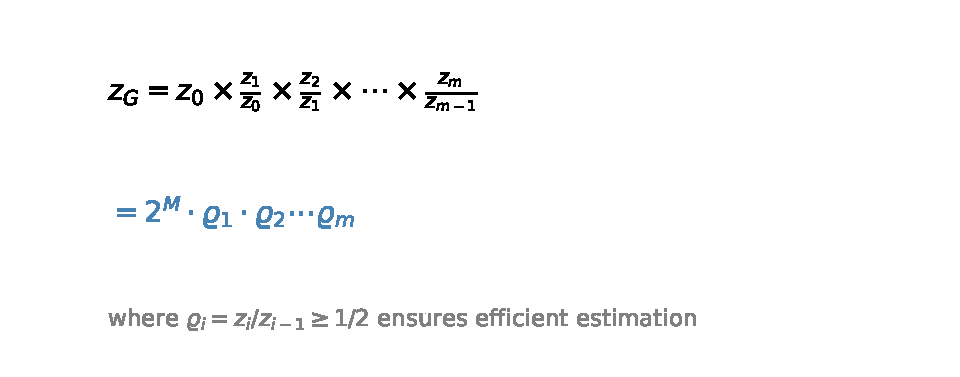
\includegraphics[width=0.80\linewidth]{fig_fpras_decomposition}

\end{frame}

\begin{frame}[allowframebreaks]{6.5.1 FPRAS for Independent Sets}

\textbf{Setup.} Let $G = (V, E)$ with $M = |V|$ vertices and $m = |E|$ edges.
Order the edges $E = \{e_1, \ldots, e_m\}$ and define the sequence of graphs $G_i = (V, E_i)$ where $E_i = \{e_1, \ldots, e_i\}$ (add one edge at a time).
Let $\Lambda_i$ = set of independent sets of $G_i$, and $z_i = |\Lambda_i|$, with $z_0 = 2^M$ (all subsets of $V$ are independent sets of the edgeless graph).

\begin{block}{Key Lemma 6.5.7: Each Ratio is at Least $1/2$}
For $1 \le i \le m$: $\varrho_i = z_i / z_{i-1} \ge 1/2$.

\textbf{Proof.}
Adding edge $e_i = \{u,v\}$ removes from $\Lambda_{i-1}$ exactly those independent sets containing \emph{both} $u$ and $v$.
Let $A$ = independent sets in $\Lambda_{i-1}$ containing both $u$ and $v$.
We claim $|A| \le z_{i-1}/2$.
Indeed, the map $\xi \mapsto \xi(v \to 0)$ (remove $v$) is an injection from $A$ into $\Lambda_{i-1} \setminus A$.
So $|A| \le z_{i-1} - |A|$, giving $|A| \le z_{i-1}/2$.
Therefore $z_i = z_{i-1} - |A| \ge z_{i-1}/2$.
\end{block}

\framebreak

\begin{block}{Algorithm 54: $(\varepsilon/(2m), \delta/m)$-FPRASC for $\varrho_i$}
\textbf{Require:} Graphs $G_{i-1}$, $G_i$; a rapidly mixing chain $(X_n^{(i-1)})$ with stationary distribution $\pi^{(i-1)}$ (uniform on $\Lambda_{i-1}$); parameters $\varepsilon, \delta, m$.
\begin{enumerate}
  \item Let $R = \frac{200m^2}{\varepsilon^2}\ln\!\left(\frac{2m}{\delta}\right)$.
  \item For $j = 1, \ldots, R$:
    \begin{enumerate}
      \item Run chain $(X_n^{(i-1)})$ for $\tau(\varepsilon/(16m))$ steps to get approximate sample $\xi$ from $\pi^{(i-1)}$.
      \item Set $\tilde{Y}_j = \mathbf{1}(\xi \in \Lambda_{G_i})$ (check if $\xi$ is still an independent set after adding edge $e_i$).
    \end{enumerate}
  \item Return $\tilde\varrho_i = \frac{1}{R}\sum_{j=1}^R \tilde{Y}_j$.
\end{enumerate}
\end{block}

\begin{block}{Algorithm 55: $(\varepsilon, \delta)$-FPRASC for $z_G$}
\begin{enumerate}
  \item For $i = 1, \ldots, m$: compute $\tilde\varrho_i$ via Algorithm 54.
  \item Return $\hat{z}_G = 2^M \prod_{i=1}^m \tilde\varrho_i$.
\end{enumerate}
\end{block}

\framebreak

\begin{block}{Proposition 6.5.4 (FPRASC Running Time)}
Let $(X_n)$ be rapidly mixing with mixing time $\tau(\kappa)$.
Then Algorithm 55 is an $(\varepsilon, \delta)$-FPRASC for $z_G$ with running time
\[
  \frac{200\,m^3}{\varepsilon^2}\ln\!\left(\frac{2m}{\delta}\right)\,\tau\!\left(\frac{\varepsilon}{16m}\right).
\]
This is polynomial in $m, 1/\varepsilon, \ln(1/\delta), \tau$.
\end{block}

\textbf{Why the union bound works.}
Each ratio is estimated with error $\le \varepsilon/(2m)$ and failure probability $\le \delta/m$.
By the union bound, all $m$ estimates are simultaneously good with probability $\ge 1 - \delta$.
A standard calculation shows the product estimator then satisfies $|\hat{z}_G/z_G - 1| \le \varepsilon$ with probability $\ge 1-\delta$.

\end{frame}

\begin{frame}[allowframebreaks]{6.5.2 Graph Colourings and Knapsack FPRAS}

The same telescoping framework applies to graph colourings and 0-1 knapsack problems.

\textbf{For graph colourings.}
Order the edges $E = \{e_1, \ldots, e_m\}$ and define $z_i$ = number of proper $r$-colourings of $G_i$.
Here $z_0 = r^M$ (all $r^M$ assignments are proper on the edgeless graph) and each ratio $\varrho_i = z_i/z_{i-1}$ must be bounded from below.

\begin{block}{Lemma 6.5.14}
If $r > 2\Delta^2$ (where $\Delta$ is the maximum degree), then $\varrho_i \ge 1/2$ for all $i$.

\textbf{Proof sketch.}
Adding edge $e_i = \{u,v\}$ removes colourings where $\xi(u) = \xi(v)$.
For a random proper colouring of $G_{i-1}$, the probability that $\xi(u) = \xi(v)$ is at most $1/(r-\Delta)$ (since $v$ has at most $\Delta$ forbidden colours).
Under the condition $r > 2\Delta^2$: $1/(r-\Delta) < 1/(2\Delta^2 - \Delta) < 1/2$.
So $\varrho_i = 1 - P(\xi(u) = \xi(v)) \ge 1/2$.
\end{block}

\framebreak

\begin{block}{Lemma 6.5.16 (FPRASC for Colourings)}
If $r > 2\Delta^2$, there exists an $(\varepsilon, \delta)$-FPRASC for the number of proper $r$-colourings with running time
\[
  \frac{200\,m^3}{\varepsilon^2}\ln\!\left(\frac{2m}{\delta}\right)\cdot\frac{r}{r - 2\Delta}\cdot M \ln\!\left(\frac{16mM}{\varepsilon}\right),
\]
where the mixing time bound $\tau(\kappa) \le \frac{r}{r-2\Delta} M \ln(M/\kappa)$ from Lemma 6.5.15 was used.
\end{block}

\textbf{For the 0-1 knapsack problem.}
Given $d$ items with weights $a_1, \ldots, a_d$ and capacity $b$, the feasible set is $\Lambda = \{\xi \in \{0,1\}^d : \sum_i a_i \xi_i \le b\}$.
A Gibbs-like sampler on a cleverly defined sequence of subproblems gives an FPRASC.

\begin{block}{Lemma 6.5.18 (Dyer et al.)}
The Gibbs sampler for the 0-1 knapsack is rapidly mixing with mixing time $O(d^{9/2+\kappa})$.
This gives an $(\varepsilon,\delta)$-FPRASC with running time polynomial in $d$, $1/\varepsilon$, and $\ln(1/\delta)$.
\end{block}

\end{frame}

% ============================================================
\section{6.6 Computational Biology: Motif Finding}
% ============================================================

\begin{frame}[allowframebreaks]{6.6 Motif Finding in DNA Sequences}

A \emph{motif} is a short, conserved sequence pattern that recurs across a collection of biological sequences.
For example, a transcription factor binding site appears at similar (but not identical) positions in the regulatory regions of co-regulated genes.

\begin{block}{Model Setup}
\begin{itemize}
  \item $k$ sequences, each of length $n$, over alphabet $\Sigma = \{A, C, G, T\}$ (encoded as $\{1,2,3,4\}$, so $d = |\Sigma| = 4$).
  \item A \emph{motif} has length $w$. In sequence $i$, the motif starts at \emph{unknown} position $\xi_i^\bullet \in \{1, \ldots, n-w+1\}$.
  \item Letters \emph{outside} the motif are generated i.i.d.\ from the \emph{background distribution} $\boldsymbol\theta_0 = (\theta_{1,0}, \ldots, \theta_{d,0})^\top$.
  \item Letters \emph{inside} the motif at column $j$ ($j = 1, \ldots, w$) are generated from the \emph{motif distribution} $\boldsymbol\theta_j = (\theta_{1,j}, \ldots, \theta_{d,j})^\top$.
  \item The \emph{position weight matrix} (PWM) is $\boldsymbol\Theta = (\boldsymbol\theta_1, \ldots, \boldsymbol\theta_w)$.
\end{itemize}
\end{block}

\framebreak

\textbf{Given:} Observed sequences $\mathbf{R} = (r_{ij})_{1 \le i \le k, 1 \le j \le n}$ and the PWM $\boldsymbol\Theta$.
\textbf{Find:} The starting positions $\boldsymbol\xi = (\xi_1, \ldots, \xi_k)$ that maximise the likelihood.

For a configuration $\boldsymbol\xi = (\xi_1, \ldots, \xi_k)$, define:
\begin{itemize}
  \item $\mathbf{A}_\xi$: the $k \times w$ matrix whose row $i$ is the motif segment of sequence $i$ starting at $\xi_i$.
  \item $\mathbf{C}_\xi$: the $d \times w$ count matrix; $\mathbf{C}_\xi(l,j)$ = number of rows $i$ where $\mathbf{A}_\xi(i,j) = l$.
  \item $\mathbf{D}_\xi$: the $d$-dimensional vector of background letter counts (letters not in any motif segment).
\end{itemize}
The complete-data likelihood factors as:
\[
  f(\boldsymbol\xi) = \underbrace{\prod_{l=1}^d \theta_{l,0}^{\mathbf{D}_\xi(l)}}_{\text{background}} \times \underbrace{\prod_{j=1}^w \prod_{l=1}^d \theta_{l,j}^{\mathbf{C}_\xi(l,j)}}_{\text{motif}}.
\]

\framebreak

To handle the combinatorial optimisation, we adopt a probabilistic approach via the \textbf{Gibbs distribution}:
\[
  \pi_\xi = \frac{1}{z(T)}\, f(\boldsymbol\xi)^{1/T} = \frac{\exp\!\left(\frac{1}{T}\log f(\boldsymbol\xi)\right)}{z(T)}.
\]
Here $T > 0$ is a \emph{temperature} parameter.
As $T \to 0$, the distribution $\pi$ concentrates on the maximisers of $f$ (the most likely starting positions).
Running a Gibbs sampler on $\pi$ with decreasing temperature implements \emph{simulated annealing}.

\begin{block}{Gibbs Sampler for Motif Finding (Algorithm 58)}
\textbf{Given:} Current configuration $\boldsymbol\xi = (\xi_1, \ldots, \xi_k)$; temperature $T$.
\begin{enumerate}
  \item Choose row $v \in \{1, \ldots, k\}$ uniformly at random.
  \item Compute the unnormalised probability of each starting position $s \in \{1, \ldots, n-w+1\}$:
        $\tilde{p}(s) \propto f(\boldsymbol\xi(v \to s))^{1/T}$.
  \item Normalise: $p(s) = \tilde{p}(s) / \sum_{r} \tilde{p}(r)$.
  \item Sample $s^* \sim p(\cdot)$ and set $\xi_v \leftarrow s^*$.
\end{enumerate}
\end{block}

\framebreak

\begin{columns}[T]
  \begin{column}{0.5\textwidth}
    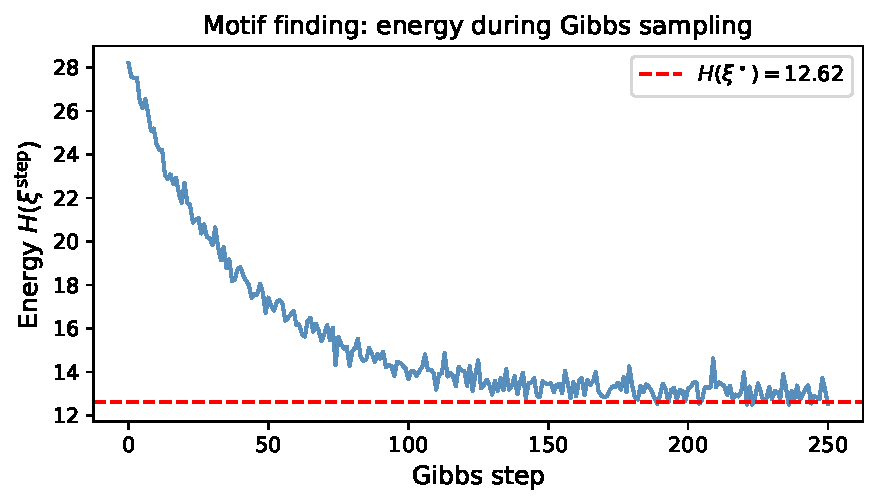
\includegraphics[width=\linewidth]{fig_motif_energy}
  \end{column}
  \begin{column}{0.46\textwidth}
    \textbf{Numerical example (Section 6.6.3).}
    Parameters: $k = 30$ sequences, $n = 20$, $w = 13$.
    True starting positions $\boldsymbol\xi^\bullet$ simulated.
    Energy $H(\boldsymbol\xi^\bullet) = -\log f(\boldsymbol\xi^\bullet) = 12.62$.

    After 200 Gibbs steps: $H(\boldsymbol\xi^{(200)}) = 12.64$.
    Only 2 of the 30 rows differ from $\boldsymbol\xi^\bullet$ (by just 1 position).
    The Gibbs sampler recovers the true motif positions reliably.
  \end{column}
\end{columns}

The key computational simplification: the ratio $\pi_{\xi(v \to s)} / \pi_{\xi(v \to r)}$ depends only on the \emph{changed} portion of $\mathbf{A}_\xi$ (row $v$), not on the entire configuration.
This makes each Gibbs step $O(kw)$ rather than $O(k \cdot n \cdot w)$.

\end{frame}

% ============================================================
\section{6.7 Estimating $I = \mathbb{E}f(X)$}
% ============================================================

\begin{frame}[allowframebreaks]{6.7 MCMC Estimation: Ergodic Theorem and CLT}

The MCMC estimator for $I = \EE_\pi f(X) = \sum_{s \in \mathcal{S}} \pi_s f(s)$ is
\[
  \hat{Y}_R = \frac{1}{R} \sum_{j=1}^{R} f(X_j),
\]
where $(X_j)_{j \ge 0}$ is an ergodic Markov chain with stationary distribution $\pi$ and $Y_j = f(X_j)$.

\begin{block}{Proposition 6.7.1 (Strong Law / Ergodic Theorem)}
If $(X_n)$ is ergodic (irreducible and aperiodic finite chain) and $f$ is real-valued, then with probability 1:
\[
  \hat{Y}_R = \frac{1}{R}\sum_{j=1}^{R} f(X_j) \xrightarrow{R \to \infty} I = \sum_{s \in \mathcal{S}} \pi_s f(s).
\]
This holds regardless of the initial distribution $\mu$.
\end{block}

\framebreak

Unlike the i.i.d.\ case, the samples $Y_1, Y_2, \ldots$ are \emph{correlated} (dependent).
This affects the variance of $\hat{Y}_R$.

\begin{block}{Proposition 6.7.5 (CLT for Markov Chains)}
If $(X_n)$ is ergodic and $f$ is real-valued, then
\[
  \sqrt{R}\,(\hat{Y}_R - I) \xrightarrow{d} \mathcal{N}(0, \varsigma^2),
\]
where the \textbf{asymptotic variance} (also called the \emph{time-average variance constant}, TAVC) satisfies
\[
  0 < \varsigma^2 = \lim_{R \to \infty} R\,\mathrm{Var}(\hat{Y}_R) < \infty.
\]
Both the limit and the CLT hold independently of the initial distribution $\mu$.
\end{block}

\framebreak

The TAVC $\varsigma^2$ can be expressed in terms of the covariances of the stationary sequence.
Let $Y_j = f(X_j)$ when $X_0 \sim \pi$, and define $\rho_k = \mathrm{Cov}(Y_0, Y_k)$.

\begin{block}{Lemma 6.7.9}
If $\bfP$ is regular, then
\[
  \mathrm{Var}(\hat{Y}_R) = \frac{1}{R}\left(1 + 2\sum_{j=1}^{R-1}\left(1 - \frac{j}{R}\right)\rho_j\right)\mathrm{Var}(Y_0),
\]
so that
\[
  \varsigma^2 = \lim_{R \to \infty} R\,\mathrm{Var}(\hat{Y}_R) = \mathrm{Var}(Y_0) + 2\sum_{k=1}^{\infty} \rho_k = \rho_0 + 2\sum_{k=1}^{\infty} \rho_k.
\]
\end{block}

The sum $\varsigma^2 = \rho_0 + 2\sum_{k\ge 1}\rho_k$ is called the \emph{spectral density at zero frequency}.
When $\rho_k < 0$ for large $k$ (negative autocorrelation), $\varsigma^2 < \mathrm{Var}(Y_0)$ and MCMC is \emph{better} than i.i.d.\ sampling.

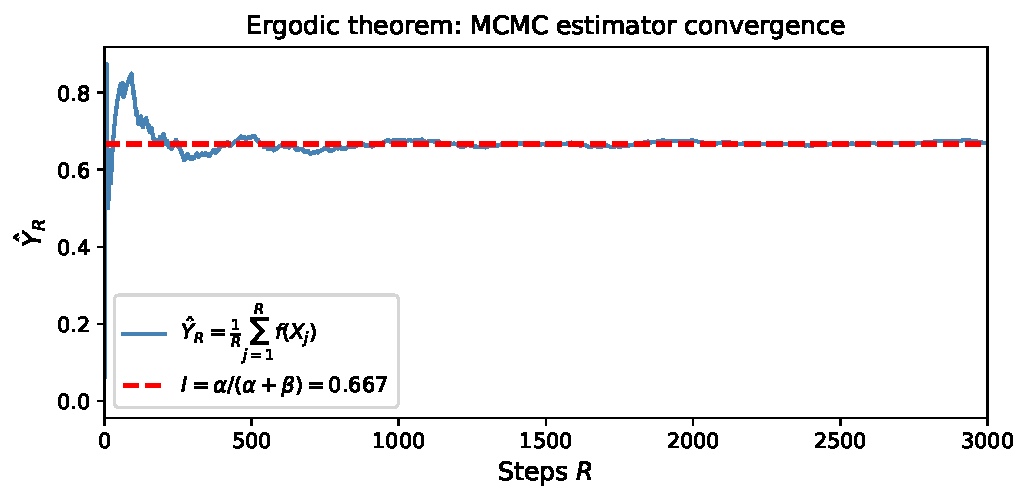
\includegraphics[width=0.85\linewidth]{fig_ergodic_convergence}

\end{frame}

\begin{frame}[allowframebreaks]{6.7 Regenerative Structure and Asymptotic Variance}

A key tool for understanding the TAVC is the \emph{regenerative structure} of ergodic Markov chains.

\textbf{Regeneration times.}
Fix a reference state $s_0 \in \mathcal{S}$ and let $\gamma_0 < \gamma_1 < \gamma_2 < \ldots$ be the successive times at which the chain visits $s_0$.
The chain \emph{regenerates} at each return to $s_0$.
The \emph{cycle lengths} $\eta_l = \gamma_l - \gamma_{l-1}$ and \emph{cycle sums} $W_l = \sum_{j=\gamma_{l-1}}^{\gamma_l - 1} f(X_j)$ are i.i.d.

\begin{block}{Representation as a Ratio of i.i.d.\ Means}
\[
  I = \lim_{R \to \infty} \hat{Y}_R = \frac{\EE[W_1]}{\EE[\eta_1]},
\]
and the TAVC satisfies
\[
  \varsigma^2 = \frac{\mathrm{Var}(W_1 - I\,\eta_1)}{\EE[\eta_1]}.
\]
This follows from the CLT for ratios of i.i.d.\ sums (Anscombe's theorem).
\end{block}

\framebreak

\begin{block}{Example 6.7.12: Two-State Chain}
Consider $\mathcal{S} = \{0,1\}$ with $\bfP = \begin{pmatrix}1-\alpha & \alpha \\ \beta & 1-\beta\end{pmatrix}$, $f(x) = x$, and reference state $s_0 = 0$.

The true value is $I = \alpha/(\alpha+\beta)$.

Cycle length: $\EE[\eta_1] = 1/\pi_0 = (\alpha+\beta)/\beta$.

Cycle sum: $W_1 = \sum_{j: X_j = 1, j < \text{return to }0} 1$.
We can show $\EE[W_1] = \alpha/\beta$ and $\mathrm{Var}(W_1 - I\eta_1) = \alpha\beta(2-\alpha-\beta)/(\alpha+\beta)^2$.

Therefore:
\[
  \varsigma^2 = \frac{\alpha\beta(2-\alpha-\beta)/(\alpha+\beta)^2}{(\alpha+\beta)/\beta} = \frac{\alpha\beta(2-\alpha-\beta)}{(\alpha+\beta)^3}.
\]

Comparison with i.i.d.\ sampling: $\mathrm{Var}(Y^{\mathrm{ind}}) = \alpha\beta/(\alpha+\beta)^2$, so
\[
  \frac{\varsigma^2}{\mathrm{Var}(Y^{\mathrm{ind}})} = \frac{2-\alpha-\beta}{\alpha+\beta}.
\]
MCMC is more efficient than i.i.d.\ when $\alpha + \beta > 1$ (fast-mixing chain).
\end{block}

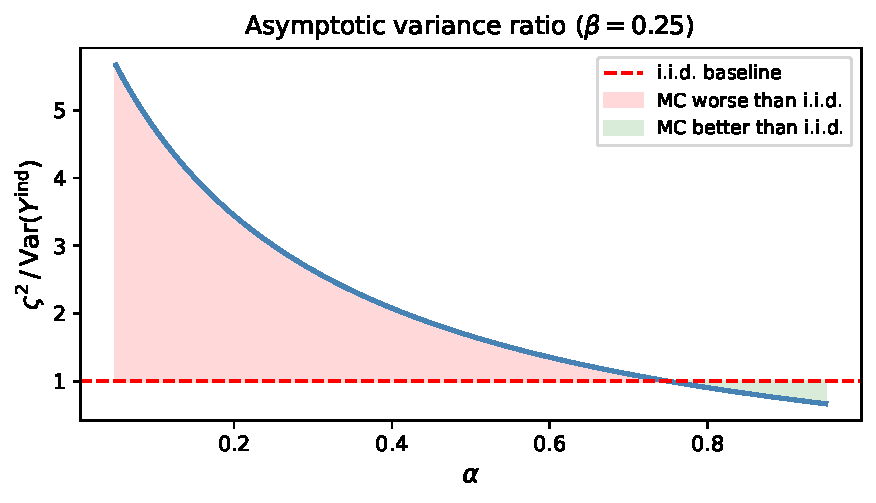
\includegraphics[width=0.75\linewidth]{fig_asymptotic_variance}

\end{frame}

\begin{frame}[allowframebreaks]{6.7 Variance Estimation and Confidence Intervals}

In practice, $\varsigma^2$ is unknown and must be estimated from the chain.
There are two main methods.

\begin{block}{Method 1: Lag Covariance Estimation}
With the chain values $Y_0, \ldots, Y_{R-1}$ (after burn-in), estimate:
\[
  \hat\rho_k = \frac{1}{R-k}\sum_{j=0}^{R-k-1}(Y_j - \hat{Y}_R)(Y_{j+k} - \hat{Y}_R), \quad k = 0, 1, \ldots, N,
\]
and
\[
  \hat\varsigma^2_N = \sum_{k=-N}^{N} \hat\rho_k = \hat\rho_0 + 2\sum_{k=1}^{N} \hat\rho_k
\]
for a truncation lag $N$ (typically $N \approx \sqrt{R}$ or chosen by an automatic rule).
\end{block}

\framebreak

\begin{block}{Method 2: Batch Means}
Divide $Y_0, \ldots, Y_{R-1}$ into $m$ non-overlapping batches of size $n$ (so $R = mn$).
The $k$-th batch mean is
\[
  \hat{Y}_k(n) = \frac{1}{n}\sum_{i=(k-1)n}^{kn-1} Y_i, \quad k = 1, \ldots, m.
\]
For $n$ large enough, $\hat{Y}_1(n), \ldots, \hat{Y}_m(n)$ are approximately i.i.d.\ $\mathcal{N}(I, \varsigma^2/n)$.
The sample variance of the batch means estimates $\varsigma^2/n$:
\[
  V_m^2(n) = \frac{1}{m-1}\sum_{k=1}^m (\hat{Y}_k(n) - \hat{Y}_R)^2.
\]
A \textbf{95\% confidence interval} for $I$ at level $1-\alpha$ is
\[
  \hat{Y}_R \pm t_{m-1,\, 1-\alpha/2} \sqrt{\frac{V_m^2(n)}{m}},
\]
where $t_{m-1,q}$ is the $q$-quantile of the $t$-distribution with $m-1$ degrees of freedom.
\end{block}

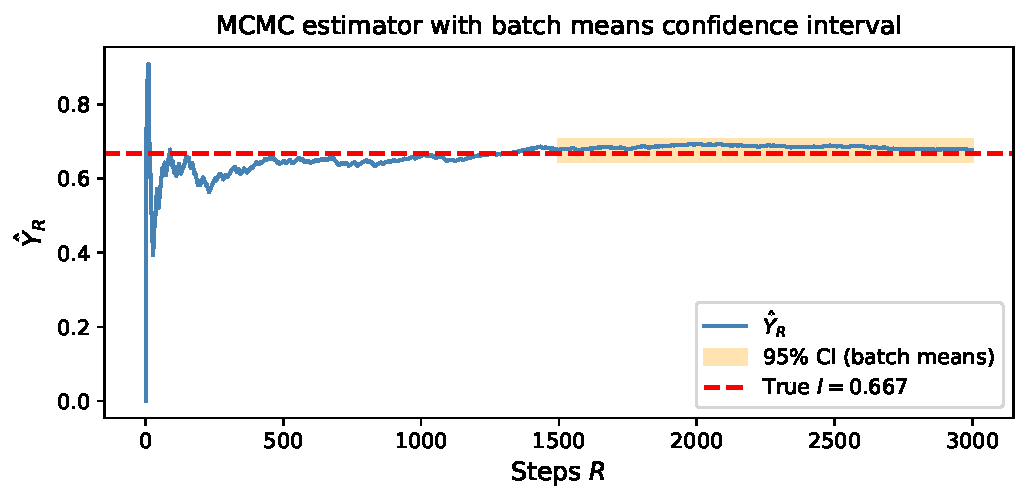
\includegraphics[width=0.75\linewidth]{fig_batch_means}

\end{frame}

\begin{frame}[fragile]{6.7 MCMC Estimation: Python Implementation}
\begin{lstlisting}[style=python]
import numpy as np
from scipy import stats

def mcmc_estimate_with_CI(chain_values, burn_in=500, n_batches=20):
    """
    Estimate I = E[f(X)] and build 95% CI using batch means.
    chain_values : array of f(X_j) from the MCMC chain
    burn_in      : number of initial samples to discard
    n_batches    : number of batches for batch means method
    """
    Y = chain_values[burn_in:]   # discard burn-in
    R = len(Y)
    I_hat = Y.mean()

    # --- Batch Means ---
    batch_size = R // n_batches
    batches = [Y[k*batch_size:(k+1)*batch_size].mean()
               for k in range(n_batches)]
    batch_std = np.std(batches, ddof=1)
    t_crit = stats.t.ppf(0.975, df=n_batches - 1)
    margin = t_crit * batch_std / np.sqrt(n_batches)

    # --- Lag covariance estimate of zeta^2 ---
    N_lag = min(250, R // 4)  # truncation lag
    Y_c = Y - I_hat
    rho_hat = np.array([np.mean(Y_c[:R-k] * Y_c[k:])
                        for k in range(N_lag + 1)])
    zeta2_hat = rho_hat[0] + 2 * rho_hat[1:].sum()

    return {
        'estimate'  : I_hat,
        'CI_lower'  : I_hat - margin,
        'CI_upper'  : I_hat + margin,
        'zeta2_hat' : zeta2_hat,
        'eff_sample': R * rho_hat[0] / zeta2_hat if zeta2_hat > 0 else R,
    }

# Two-state chain example: alpha=0.3, beta=0.1
# True I = alpha/(alpha+beta) = 0.75
alpha, beta = 0.3, 0.1
chain = [0]
for _ in range(10000):
    x = chain[-1]
    r = np.random.rand()
    if x == 0: chain.append(1 if r < alpha else 0)
    else:      chain.append(0 if r < beta  else 1)
f_vals = np.array(chain, dtype=float)  # f(x) = x
res = mcmc_estimate_with_CI(f_vals)
print(f"I_hat = {res['estimate']:.4f} (true = 0.75)")
print(f"95% CI = ({res['CI_lower']:.4f}, {res['CI_upper']:.4f})")
print(f"TAVC estimate zeta^2 = {res['zeta2_hat']:.4f}")
print(f"Effective sample size = {res['eff_sample']:.1f}")
\end{lstlisting}
\end{frame}

\begin{frame}[allowframebreaks]{6.7 Hard-core Model: Worked Numerical Example}

We illustrate the full estimation pipeline on the hard-core model from Example 6.7.13 in the book.

\textbf{Setup.} Grid graph $G = (\{1,\ldots,8\}^2, E)$ with $M = 64$ vertices and $\lambda = 2$.
Quantity of interest: $I = \EE_\pi m(\xi) = \EE_\pi[\text{number of occupied vertices}]$.

\textbf{Chain.} Gibbs sampler (Algorithm 47) run for $R = 10{,}000$ steps after a burn-in of $k_0 = 500$ steps.
The TAVC is estimated by lag-$k$ covariances with truncation lag $N = 250$.

\textbf{Results (from the book, Table 6.2).}
\begin{itemize}
  \item $\hat{Y}_R \approx 24.37$ (estimated mean number of particles).
  \item Lag-covariance estimate: $\hat\varsigma^2 \approx 8.42$.
  \item 95\% confidence interval: $(23.15,\, 25.59)$.
\end{itemize}

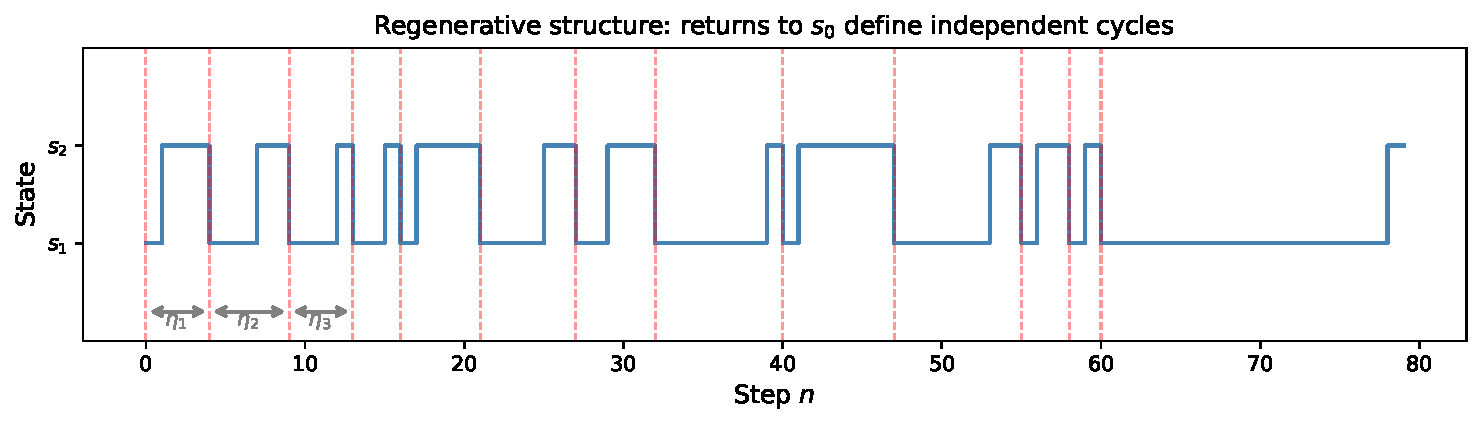
\includegraphics[width=0.85\linewidth]{fig_regenerative}

\begin{alertblock}{Key Takeaway}
The asymptotic variance $\varsigma^2 \approx 8.42$ is much larger than $\mathrm{Var}(Y_0) = \rho_0$ for i.i.d.\ samples, reflecting the positive autocorrelation in the Gibbs chain.
The effective sample size is $R \cdot \rho_0 / \varsigma^2 \ll R$; MCMC samples are ``worth less'' than i.i.d.\ samples in this example because the chain mixes slowly near the phase transition.
\end{alertblock}

\end{frame}

% ============================================================
\section{6.8 Stable Simulation Scheme}
% ============================================================

\begin{frame}[allowframebreaks]{6.8 Stable Simulation: Estimating $\pi(A)$ Exactly}

In some applications we want to estimate the stationary probability $\pi(A) = \sum_{s \in A} \pi_s$ for a specific set $A$, with \emph{exact} (not approximate) samples from $\pi$.
The naive approach --- generate MCMC samples and estimate $\pi(A) \approx \frac{1}{R}\sum_{j=1}^R \mathbf{1}(X_j \in A)$ --- requires dealing with burn-in.
The \emph{stable simulation scheme} avoids this using \emph{Siegmund duality}.

\textbf{Setting.} $\mathcal{S} = \{s_1, \ldots, s_m\}$ is partially ordered by $\preceq$.
For a state $s_j$, we want to estimate
\[
  \pi(\{s_j\}^\downarrow) = \pi\bigl(\{s' : s' \preceq s_j\}\bigr).
\]

\begin{block}{Definition 6.8.1 (Siegmund Dual)}
The Markov chain $(Z_n)$ with transition matrix $\bfP_Z$ on $\mathcal{S}^* = \{s_0\} \cup \mathcal{S}$ is the \textbf{Siegmund dual} of $(X_n)$ with t.m.\ $\bfP_X$ if
\[
  \bfP_X^n(s_i, \{s_j\}^\downarrow) = \bfP_Z^n(s_j, \{s_i\}^\uparrow) \quad \forall\, s_i, s_j \in \mathcal{S},\; n \ge 0.
\]
\end{block}

\framebreak

Taking $n \to \infty$: since $(X_n)$ is ergodic, $\bfP_X^n(s_i, \{s_j\}^\downarrow) \to \pi(\{s_j\}^\downarrow)$ for any starting state $s_i$.
Also, $\bfP_Z^n(s_j, \{s_i\}^\uparrow) \to \PP(Z \text{ absorbed in } s_m \mid Z_0 = s_j)$ as the state $s_0$ acts as an absorbing boundary.
Therefore:
\[
  \pi(\{s_j\}^\downarrow) = \PP(Z \text{ absorbed at } s_m \mid Z_0 = s_j).
\]
This is the key formula: the stationary probability of a down-set equals the absorption probability of the dual chain.

\begin{block}{Algorithm 59 (Stable Simulation Scheme)}
\textbf{Require:} Chain $(X_n)$ on $\mathcal{S}$; its Siegmund dual $(Z_n)$ on $\mathcal{S}^*$; desired set $\{s_j\}^\downarrow$; replications $R$.
\begin{enumerate}
  \item Compute the Siegmund dual $\bfP_Z$ of $\bfP_X$ on $\mathcal{S}^* = \{s_0\} \cup \mathcal{S}$.
  \item For $l = 1, \ldots, R$: simulate $(Z_n^{(l)})$ starting from $s_j$ until absorption at $s_0$ or $s_m$.
  \item Estimate: $\hat\pi(\{s_j\}^\downarrow) = \frac{1}{R}\sum_{l=1}^R \mathbf{1}(Z^{(l)} \text{ absorbed at } s_m)$.
\end{enumerate}
The $R$ simulations are i.i.d., so the estimator is unbiased, and $R \approx (1.96/b)^2$ gives a 95\% CI of half-width $b$.
\end{block}

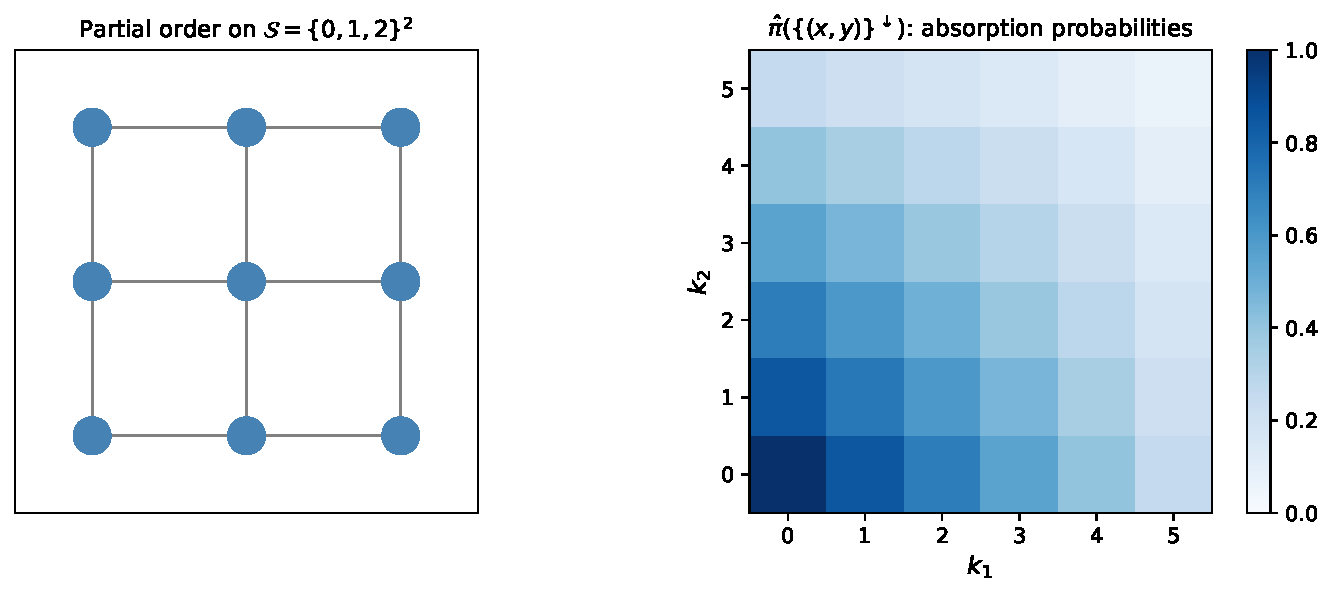
\includegraphics[width=0.75\linewidth]{fig_siegmund_duality}

\framebreak

\begin{block}{Definition (Möbius Monotonicity) and Lemma 6.8.2}
A chain $(X_n)$ with t.m.\ $\bfP_X$ is \textbf{Möbius monotone} w.r.t.\ $\preceq$ if the matrix $\mathbf{C}^{-1} \bfP_X \mathbf{C} \ge 0$, where $\mathbf{C}(s_i, s_j) = \mathbf{1}(s_i \preceq s_j)$ is the ordering matrix and $\mathbf{C}^{-1}$ is its inverse (the Möbius function).

A Siegmund dual on $\mathcal{S}^*$ exists if and only if $(X_n)$ is Möbius monotone w.r.t.\ $\preceq$.
\end{block}

\begin{block}{Example 6.8.4: Two-Node Tandem Queue}
Two-node closed tandem queue with state space $\mathcal{S} = \{0,\ldots,N\}^2$, parameters $\lambda_1, \lambda_2$ (arrival rates) and $\mu_1, \mu_2$ (service rates).
For $N = 5$, $\lambda_1 = 3/16$, $\lambda_2 = 1/16$, $\mu_1 = \mu_2 = 6/16$, and $R = 4 \times 10^4$ replications:

\medskip
\begin{center}
\footnotesize
\begin{tabular}{c|cccccc}
  \toprule
  $y \backslash x$ & 0 & 1 & 2 & 3 & 4 & 5 \\
  \midrule
  0 & 0.030 & 0.081 & 0.145 & 0.236 & 0.351 & 0.502 \\
  1 & 0.058 & 0.139 & 0.249 & 0.381 & 0.550 & 0.763 \\
  2 & 0.079 & 0.181 & 0.310 & 0.468 & 0.652 & 0.884 \\
  3 & 0.094 & 0.207 & 0.353 & 0.511 & 0.710 & 0.946 \\
  4 & 0.102 & 0.224 & 0.372 & 0.540 & 0.743 & 0.981 \\
  5 & 0.111 & 0.235 & 0.383 & 0.558 & 0.762 & 1.000 \\
  \bottomrule
\end{tabular}
\end{center}
Estimates of $\hat\pi(\{(x,y)\}^\downarrow)$ for all $(x,y) \in \{0,\ldots,5\}^2$. Each entry is unbiased.
\end{block}

\end{frame}

% ============================================================
\section{6.9 Bibliographical Notes}
% ============================================================

\begin{frame}[allowframebreaks]{6.9 Bibliographical Notes}

The field of MCMC has a rich history spanning physics, statistics, and computer science.

\begin{block}{Foundational References}
\begin{itemize}
  \item \textbf{Markov chain theory:} Norris [165] is a clear introductory textbook; Meyn \& Tweedie [147] provide a comprehensive treatment including general state spaces.
  \item \textbf{Metropolis algorithm:} Introduced by Metropolis, Rosenbluth, Rosenbluth, Teller \& Teller [145] (1953) for molecular dynamics simulations. Generalised to asymmetric proposals by Hastings [78] (1970).
  \item \textbf{Gibbs sampler:} Introduced by Geman \& Geman [62] (1984) for image restoration via simulated annealing. Popularised in Bayesian statistics by Gelfand \& Smith [61] (1990).
  \item \textbf{Coupling from the Past:} Propp \& Wilson [170] (1996) introduced the CFTP algorithm. The monotone version using only min/max chains is due to Huber [85].
\end{itemize}
\end{block}

\begin{block}{FPRAS and Approximate Counting}
\begin{itemize}
  \item The general FPRAS framework via self-reducibility: Jerrum, Valiant \& Vazirani [100].
  \item Rapid mixing of the Gibbs sampler for graph colourings with $r \ge 2\Delta+1$: Jerrum [99] (1995).
  \item Rapid mixing for 0-1 knapsack: Dyer, Frieze \& Kannan [43].
  \item Rapid mixing via the Metropolis algorithm for $r \ge 2\Delta+1$ colours: Hayes [85].
\end{itemize}
\end{block}

\begin{block}{Ergodic Theory and Variance Estimation}
\begin{itemize}
  \item CLT for Markov chains: Meyn \& Tweedie [147]; Glynn \& Iglehart [64].
  \item Batch means for variance estimation: Damerdji [30]; Alexopoulos \& Seila [4].
  \item Regenerative simulation: Crane \& Iglehart; see also Glynn \& Iglehart [64].
\end{itemize}
\end{block}

\begin{block}{Other Topics}
\begin{itemize}
  \item Motif finding via Gibbs sampling: Lawrence \emph{et al.}\ [119]; Liu, Neuwald \& Lawrence [128].
  \item Siegmund duality and stable simulation: Siegmund [191]; Lorek \& Szekli [130].
  \item Ising model and critical phenomena: see textbooks by Grimmett [68] or Georgii [63].
\end{itemize}
\end{block}

\end{frame}

% ============================================================
\section{6.10 Selected Exercises}
% ============================================================

\begin{frame}[allowframebreaks]{6.10 Selected Exercises}

\begin{block}{Exercise 6.T.7 (Riffle Shuffle)}
Let $(X_k)$ be a Markov chain on $\mathcal{S} = S_n$ (permutations of $n$ elements) corresponding to the Riffle Shuffle, and let $(\hat{X}_k)$ be its time-reversal.
Show that
\[
  \forall\, \mu,\; \forall\, k \ge 0: \quad \dTV(\mu \bfP_X^k, \pi) = \dTV(\mu \bfP_{\hat X}^k, \pi),
\]
where $\pi$ is the uniform distribution on $S_n$.
\end{block}

\begin{block}{Exercise 6.T.8 (Total Variation Distance)}
Show that for two probability vectors $\bfmu$ and $\bfv$ on $\mathcal{S}$:
\[
  \dTV(\bfmu, \bfv) = \max_{A \subseteq \mathcal{S}}|\mu(A) - \nu(A)|.
\]
\textit{Hint:} Take $A = \{s : \mu_s > \nu_s\}$ to show $\ge$; use the triangle inequality for $\le$.
\end{block}

\begin{block}{Exercise 6.T.12 (Los Angeles Weather Chain)}
Consider $\mathcal{S} = \{\text{rainy}, \text{sunny}\}$ with $\bfP = \begin{pmatrix}1/2 & 1/2 \\ 1/10 & 9/10\end{pmatrix}$.
\begin{enumerate}[(a)]
  \item Find the stationary distribution.
  \item Starting from the ``rainy'' state, compute $\dTV(\bfmu \bfP^n, \pi)$ for $n = 1, 2, 3$.
\end{enumerate}
\textit{Solution for (a):} Solve $\pi_r/2 + \pi_s/10 = \pi_r$. With $\pi_r + \pi_s = 1$: $\pi_r = 1/6$, $\pi_s = 5/6$.
\end{block}

\framebreak

\begin{block}{Exercise 6.T.20 (Gibbs as Special Case of MH)}
Show that the Gibbs sampler (Algorithm 44) is a special case of the Metropolis-Hastings algorithm (Algorithm 43) with acceptance ratio always equal to 1.

\textit{Hint:} For the Gibbs proposal, what is $q_{\xi\xi'}/q_{\xi'\xi}$ when $\xi$ and $\xi'$ differ at exactly one vertex $v$?
\end{block}

\begin{block}{Exercise 6.T.24 (Coupling Not Sufficient for Stationarity)}
Consider a two-state chain $\mathcal{S} = \{1,2\}$ that with probability 1 stops in state 1 (state 1 is absorbing, state 2 transitions to 1).
The forward coupling time $\tau_f = \min\{n : X_n = X'_n\}$ is finite with probability 1.
Show that $X_{\tau_f}^0$ is NOT distributed as $\pi$ (where $\pi$ would be the uniform distribution if the chain were ergodic).
\textit{This illustrates why CFTP must run \emph{backward} from the past, not forward from the present.}
\end{block}

\begin{block}{Exercise 6.T.35 (Median Trick for Boosting)}
If $p > 1/2$ and $Y_1, \ldots, Y_R \overset{i.i.d.}{\sim} \mathrm{Bernoulli}(p)$, show that
\[
  \PP\!\left(\sum_{i=1}^R Y_i > R/2\right) \ge 1 - \delta \quad \text{when } R \ge \frac{\ln(1/\delta)}{2(p-1/2)^2}.
\]
\textit{This result (via Chebyshev or Hoeffding) underlies the FPRAS boosting argument.}
\end{block}

\end{frame}

% ============================================================
% Chapter Summary
% ============================================================

\begin{frame}[allowframebreaks]{Chapter 6 Summary}

Chapter 6 developed the theory and practice of Markov Chain Monte Carlo (MCMC) from the ground up.

\begin{block}{Core Algorithms and Their Applications}
\begin{tabular}{lll}
\toprule
Algorithm & Section & Application \\
\midrule
Metropolis (Alg.~42) & 6.3.1 & Symmetric proposal, any $\pi$ \\
Metropolis-Hastings (Alg.~43) & 6.3.1 & Asymmetric proposal, any $\pi$ \\
Gibbs Sampler (Alg.~44--48) & 6.3.2 & Product space, full conditionals \\
CFTP -- general (Alg.~49) & 6.4.1 & Exact sampling \\
CFTP -- monotone (Alg.~50) & 6.4.3 & Efficient exact sampling \\
FPRAS (Alg.~54--55) & 6.5.1 & Approximate counting \\
Motif Gibbs (Alg.~58) & 6.6 & Bioinformatics motif finding \\
Stable Simulation (Alg.~59) & 6.8 & Exact $\pi(A)$ via duality \\
\bottomrule
\end{tabular}
\end{block}

\framebreak

\begin{block}{Key Theoretical Results}
\begin{enumerate}
  \item \textbf{DBC implies stationarity:} If $w_s p_{ss'} = w_{s'} p_{s's}$ for all $s,s'$, then $\pi_s \propto w_s$ is stationary.
  \item \textbf{Ergodic theorem (Prop.~6.7.1):} $\hat{Y}_R \to I$ a.s.\ for any ergodic chain.
  \item \textbf{CLT (Prop.~6.7.5):} $\sqrt{R}(\hat{Y}_R - I) \xrightarrow{d} \mathcal{N}(0,\varsigma^2)$ with $\varsigma^2 = \rho_0 + 2\sum_{k \ge 1}\rho_k$.
  \item \textbf{CFTP correctness (Thm.~6.4.2):} Backward coupling from all initial states yields exact sample from $\pi$.
  \item \textbf{FPRAS (Prop.~6.5.4):} Telescoping ratios $z_i/z_{i-1} \ge 1/2$ + rapid mixing $\Rightarrow$ polynomial-time approximate counter.
  \item \textbf{Siegmund duality (Eq.~6.8.2):} $\pi(\{s_j\}^\downarrow) = P(Z \text{ absorbed at } s_m \mid Z_0 = s_j)$.
\end{enumerate}
\end{block}

\begin{alertblock}{The MCMC Paradigm in One Sentence}
Build a Markov chain with stationary distribution $\pi$ that only requires computing ratios $\pi_{s'}/\pi_s$; run it; average the output; the normalising constant never appears.
\end{alertblock}

\end{frame}

\end{document}
